%% Vol III, Chapter 2 — Mathematical Companion
%% SOURCE: docs/working/papers/SSRN_companion/Math_Companion_SSRN.tex (full LaTeX source)
%%         docs/working/papers/SSRN_companion/figures/ (7 figure PDFs)

\chapter{Mathematical Companion}
\label{vol3:chap:math}

%% TODO(bob): this chapter is a formal reference for the mathematical and
%% engineering structures described in Math_Companion_SSRN.tex.
%% The full source is available at:
%%   docs/working/papers/SSRN_companion/Math_Companion_SSRN.tex
%%
%% Option A: include it directly:
%%   % Moved from docs/SSRN_companion/Math_Companion_SSRN.tex to docs/working/papers/SSRN_companion/Math_Companion_SSRN.tex on 2026-06-16 (docs reorg Phase 2)
% ============================================================================
% MATHEMATICAL AND ENGINEERING STRUCTURES OF THE STARFORTH RUNTIME
%
% A Companion Document to:
%   "Steady-State Convergence in a Self-Adaptive Virtual Machine:
%    An Empirical Study"  (SSRN, James 2025)
%
% Inventor / Author: Robert A. James
% Repository:        github.com/rajames440/StarForth
% Branch:            claude/math-structures-ssrn-KzJyq
%
% This companion mines the entire StarForth repository --- not just the SSRN
% paper --- and presents every mathematical and engineering structure that
% governs the runtime, in a single math-first reference. Every formula is
% cross-referenced to its implementation. Every constant is cross-referenced
% to its measured value. Every conjecture is stated explicitly.
% ============================================================================

\documentclass[11pt,letterpaper,openany]{book}

% ---------- packages ----------
\usepackage[utf8]{inputenc}
\usepackage[T1]{fontenc}
\usepackage{lmodern}
\usepackage[margin=1in]{geometry}
\usepackage{graphicx}
\usepackage{float}
\usepackage{placeins}
\usepackage{amsmath}
\usepackage{amssymb}
\usepackage{amsthm}
\usepackage{mathtools}
\usepackage{booktabs}
\usepackage{longtable}
\usepackage{array}
\usepackage{enumitem}
\usepackage{xcolor}
\usepackage{listings}
\usepackage{algorithm}
\usepackage{microtype}
\usepackage[hidelinks,colorlinks=true,linkcolor=blue!60!black,citecolor=blue!60!black,urlcolor=blue!60!black]{hyperref}
\usepackage{fancyhdr}
\usepackage{tabularx}
\usepackage{textcomp}
\usepackage{xspace}

\graphicspath{{figures/}}

% ---------- listings (C code) ----------
\definecolor{codebg}{rgb}{0.97,0.97,0.95}
\definecolor{codekw}{rgb}{0.12,0.32,0.70}
\definecolor{codestr}{rgb}{0.40,0.20,0.10}
\definecolor{codecom}{rgb}{0.30,0.50,0.30}
\definecolor{codenum}{rgb}{0.55,0.55,0.55}

\lstdefinestyle{cstyle}{
  backgroundcolor=\color{codebg},
  basicstyle=\ttfamily\footnotesize,
  keywordstyle=\color{codekw}\bfseries,
  commentstyle=\color{codecom}\itshape,
  stringstyle=\color{codestr},
  numberstyle=\color{codenum}\tiny,
  numbers=left,
  numbersep=6pt,
  frame=single,
  framerule=0.3pt,
  rulecolor=\color{gray!50},
  showstringspaces=false,
  breaklines=true,
  breakatwhitespace=true,
  language=C,
  morekeywords={uint8_t,uint16_t,uint32_t,uint64_t,int8_t,int16_t,int32_t,int64_t,size_t,cell_t,vaddr_t,q48_16_t,VM,DictEntry,RollingWindowOfTruth,HotwordsCache,WordTransitionMetrics,HeartbeatState,HeartbeatSnapshot,HeartbeatTickSnapshot,InferenceInputs,InferenceOutputs,ssm_l8_mode_t,ssm_l8_state_t,ssm_l8_metrics_t,ssm_config_t,DictPhysics,word_func_t,PipelineGlobalMetrics,BayesianLatencyPosterior,HotwordsStats,sf_mutex_t},
  captionpos=b,
  belowcaptionskip=4pt
}
\lstset{style=cstyle}

% ---------- theorem environments ----------
\theoremstyle{definition}
\newtheorem{definition}{Definition}[chapter]
\newtheorem{convention}[definition]{Convention}
\newtheorem{remark}[definition]{Remark}
\newtheorem{example}[definition]{Example}
\newtheorem{construction}[definition]{Construction}

\theoremstyle{plain}
\newtheorem{theorem}[definition]{Theorem}
\newtheorem{proposition}[definition]{Proposition}
\newtheorem{lemma}[definition]{Lemma}
\newtheorem{corollary}[definition]{Corollary}
\newtheorem{empiricallaw}[definition]{Empirical Law}
\newtheorem{openconjecture}[definition]{Conjecture}
\newtheorem{invariant}[definition]{Invariant}

% ---------- epistemic-status badges (claim provenance) ----------
% Every quantitative claim in this companion is tagged with one of four
% levels of empirical support. The badge appears INLINE before the claim.
%
%   \confirmed  : empirically validated AND replicated. Example: K = 1.0 in
%                 355 window-scaling runs with |K-1| = 0 to all digits.
%   \likely     : strong empirical evidence but one campaign or limited
%                 replication. Example: omega_0 = 934 Hz on x86_64 only.
%   \hinted     : single observation, suggestive but not replicated.
%                 Example: golden-ratio tick ratio at DIVERSE tick 13.
%   \conjecture : proposed but untested OR derived analogy without
%                 confirming experiment.
\newcommand{\confirmed}{\textcolor{green!50!black}{\textbf{[CONFIRMED]}}\xspace}
\newcommand{\likely}{\textcolor{blue!60!black}{\textbf{[LIKELY]}}\xspace}
\newcommand{\hinted}{\textcolor{orange!75!black}{\textbf{[HINTED]}}\xspace}
\newcommand{\conjecture}{\textcolor{red!60!black}{\textbf{[CONJECTURE]}}\xspace}

% ---------- math shortcuts ----------
\newcommand{\Qfp}{\mathbb{Q}_{48.16}}                % the Q48.16 number system
\newcommand{\Lambdaeff}{\Lambda_{\mathrm{eff}}}
\newcommand{\Wact}{W_{\mathrm{actual}}}
\newcommand{\Wcfg}{W_{\mathrm{config}}}
\newcommand{\Weff}{W_{\mathrm{eff}}}
\newcommand{\Wmax}{W_{\mathrm{max}}}
\newcommand{\Wmin}{W_{\mathrm{min}}}
\newcommand{\Teff}{T_{\mathrm{eff}}}
\newcommand{\E}{\mathbb{E}}
\newcommand{\Var}{\operatorname{Var}}
\newcommand{\CV}{\operatorname{CV}}
\newcommand{\diag}{\operatorname{diag}}
\newcommand{\dom}{\operatorname{dom}}
\newcommand{\codom}{\operatorname{cod}}
\newcommand{\heat}{H}
\newcommand{\Loop}[1]{L_{#1}}
\newcommand{\sourceref}[2]{\texttt{#1}:\texttt{#2}}

% ---------- page style ----------
\pagestyle{fancy}
\fancyhf{}
\fancyhead[LE]{\nouppercase{\leftmark}}
\fancyhead[RO]{\nouppercase{\rightmark}}
\fancyfoot[C]{\thepage}
\renewcommand{\headrulewidth}{0.3pt}
\setlength{\headheight}{14.5pt}

\title{
  \vspace{-2.5em}
  \textbf{\Huge Mathematical and Engineering}\\[0.2em]
  \textbf{\Huge Structures of the StarForth Runtime}\\[1.0em]
  {\Large A Treasure-Trove Reference Companion to}\\[0.3em]
  {\large\itshape ``Steady-State Convergence in a Self-Adaptive
    Virtual Machine: An Empirical Study''}\\[0.3em]
  {\large\itshape (SSRN, James 2025)}
}
\author{
  \textbf{Robert A. James}\\
  {\small \texttt{star.4th@proton.me}}\\
  {\small Independent Researcher}
}
\date{\today}

% ============================================================================
\begin{document}
\frontmatter
\maketitle
\thispagestyle{empty}

\vfill
\noindent\textbf{About this document.} This companion exists to make the
mathematics of the StarForth steady-state runtime \emph{available} ---
gathered, named, indexed, cross-referenced to code, and presented in one
place. The SSRN paper documents what was measured. This companion documents
\emph{the formal apparatus inside which those measurements live}: the state
space, the operators, the statistical machinery, the conservation law, the
sixteen-mode supervisory controller, the eleven-dimensional phase space,
and the seven feedback loops on which all of it rides.

\medskip
\noindent The boast is short, and it is meant: \textbf{every equation that
follows is grounded either in implemented code or in a measured experiment}
(38{,}935 runs, three independent campaigns). The hedging in the SSRN paper
is preserved in the main body. The conjectures appendix is where the
provocations live --- the targets we'd love to see a mathematician knock
down or upgrade.

\medskip
\noindent\textbf{How to read it.}
\begin{itemize}\setlength\itemsep{0pt}
  \item If you are a \emph{mathematician}: jump to Chapter~\ref{ch:james-law}
    (James Law) and Appendix~\ref{app:conjectures} (open conjectures).
  \item If you are a \emph{systems engineer}: jump to
    Chapter~\ref{ch:state-space} (state space) and Chapter~\ref{ch:loops}
    (the seven feedback loops).
  \item If you are a \emph{statistician}: jump to Chapter~\ref{ch:inference}
    (the inference engine).
  \item If you are a \emph{physicist}: jump to Chapter~\ref{ch:phase-space}
    (phase space and attractor dynamics).
\end{itemize}

\noindent Source citations use the form \sourceref{include/vm.h}{339}.
All file paths are relative to the repository root.

\vfill
\noindent\textit{Companion document --- not the SSRN submission itself.\\
The SSRN paper is \texttt{papers/James\_Steady-State\_Convergence\_Adaptive\_Runtime.pdf}.}
\clearpage

\tableofcontents
\clearpage

% ============================================================================
\chapter*{Notation}
\addcontentsline{toc}{chapter}{Notation}
\label{ch:notation}

\begin{longtable}{@{}p{0.18\textwidth}p{0.78\textwidth}@{}}
\toprule
\textbf{Symbol} & \textbf{Meaning} \\
\midrule
\endfirsthead
\toprule \textbf{Symbol} & \textbf{Meaning} \\ \midrule \endhead
$\Qfp$            & Q48.16 fixed-point number system; \texttt{uint64\_t} with 16 fractional bits. \\
$K$               & Dimensionless stability statistic ($K$-signal). \\
$\Lambdaeff$      & Intrinsic characteristic wavelength; measured at $256$ bytes. \\
$W$, $\Wcfg$      & Configured rolling-window size (bytes). \\
$\Wact$           & Effective (actually utilised) window size. \\
$\Weff$           & Adaptive window size at runtime, $\Wmin \le \Weff \le \Wmax$. \\
$\heat_w$, $H_w$  & Execution heat of dictionary entry $w$ (heat units, integer). \\
$H_{\mathrm{total}}$ & Aggregate heat $\sum_w H_w$. \\
$S$, $S_H$        & Shannon entropy of the heat distribution. \\
$\lambda$         & Heat-decay rate (per microsecond, Q48.16). \\
$\sigma_t^2$      & Variance of execution-time measurements across replicates. \\
$\CV$             & Coefficient of variation, $\sigma/\mu$. \\
$f_0$, $\omega_0$ & Natural frequency / circular frequency of the runtime. \\
$\phi$            & Phase offset (paper); also golden ratio $\approx 1.618$ (framework). \\
$\Teff$           & Effective temperature of a workload (Boltzmann fit). \\
$\gamma$          & Damping coefficient (per tick). \\
$\Omega$          & Ringing angular frequency (per tick). \\
$\tau$            & Relaxation time, $\tau = 1/\gamma$. \\
$\mathrm{DoF}$    & Degrees of freedom (number of active feedback loops). \\
$\Loop{i}$        & The $i$-th feedback loop, $i \in \{1,\dots,7\}$. \\
$\Loop{8}$        & The Jacquard mode selector (supervisory controller). \\
$\mathbb{F}_2^7$  & Loop-configuration lattice; $|\mathbb{F}_2^7|=128$. \\
$N$               & Number of dictionary entries. \\
$P(a\to b)$       & Transition probability from word $a$ to word $b$. \\
$\sf_M$           & Mode-selector mapping $\sf_M:\;(\text{entropy},\CV,\text{temporal}) \to \{C_0,\dots,C_{15}\}$. \\
\bottomrule
\end{longtable}

\clearpage

% ============================================================================
\chapter*{Epistemic Status of Claims}
\addcontentsline{toc}{chapter}{Epistemic Status of Claims}
\label{ch:epistemic}

This companion makes hundreds of quantitative claims. Each one carries a
provenance badge, set as the first text of the claim:

\begin{table}[H]
  \centering
  \small
  \begin{tabular}{p{0.18\textwidth} p{0.78\textwidth}}
    \toprule
    Badge & Meaning \\
    \midrule
    \confirmed       & Empirically validated \emph{and} replicated. Multiple
                       independent runs, an explicit hypothesis test, and
                       a published $p$-value or zero residual.
                       Example: ``$K = 1.0$ across 355 window-scaling runs,
                       $|K-1| = 0$ to all digits measured.'' \\[0.4em]
    \likely          & Strong empirical evidence but limited in scope ---
                       single campaign, single hardware, or
                       campaign-specific instrumentation.
                       Example: ``$\omega_0 = 934$\,Hz word-level invariance
                       on Intel N150.'' \\[0.4em]
    \hinted          & Single observation, suggestive but not replicated.
                       Reported here for completeness; needs a dedicated
                       experiment to confirm. Example: ``DIVERSE workload
                       tick ratio of $1.583\approx\varphi$ at tick 13.'' \\[0.4em]
    \conjecture      & Proposed but not yet tested, derived by analogy to
                       physical systems, or stated as an open invitation to
                       formalize. All entries in
                       Appendix~\ref{app:conjectures} carry this badge. \\
    \bottomrule
  \end{tabular}
  \caption{Provenance taxonomy for claims in this companion.}
\end{table}

\noindent\textbf{Reading rule.} If a claim has no badge it is either a
definition (in which case no provenance is required) or a derivation from
previously badged claims (in which case the strength of the conclusion is
the \emph{minimum} of the badges in its premises).

\noindent\textbf{Retroactive tags for Chapter~\ref{ch:exec-summary}.}
\begin{itemize}\setlength\itemsep{0pt}
  \item \confirmed The dimensionless statistic $K$ exhibits $\CV < 1\%$ for
        most configurations (SSRN \S4, 38{,}400 runs).
  \item \confirmed The empirical relation
        $K(W) = \Lambdaeff/W \cdot [1+A(W)\sin(2\pi f_0\log_2 W + \phi)]$
        fits with $R^2 > 0.99$ (SSRN \S6.3, $p<0.0001$).
  \item \confirmed $K \equiv 1.0$ exactly in the window-scaling form
        $K = \Lambdaeff(\mathrm{DoF}+1)/W$ across $355$ runs
        (Framework \S4.2).
  \item \confirmed $\Lambdaeff = 256\pm 8$ bytes; $f_0 = 0.667\pm 0.02$
        cycles/window doubling (FFT spectral peak, $p<10^{-4}$).
  \item \confirmed Zero variance ($\sigma = 0$, $S = 0$) at the triple-lock
        window $W = 4096$ across all $30$ replicates (Patent Table~3).
  \item \confirmed Bimodal $K$ distribution at $W \in \{6144, 16384\}$ with
        $47/53\%$ split (Patent Table~4).
  \item \likely    $\omega_0 = 934$\,Hz word-level invariance: $\CV = 0.14\%$
        across $355$ runs on Intel N150 (one hardware platform).
  \item \likely    $\omega_0 = 13.6$\,Hz heartbeat-level (180 runs, one
        hardware platform).
  \item \hinted    Golden ratio tick-ratio $1.583\approx\varphi$ at
        DIVERSE tick 13 (single observation, Framework \S4.4).
  \item \conjecture $\Lambdaeff$ is a hardware constant equal to $4\times$
        cache-line size (Conjecture C1, Appendix~\ref{app:conjectures}).
\end{itemize}

\medskip
\noindent\textbf{Retroactive tags for Chapter~\ref{ch:boltzmann}.}
\begin{itemize}\setlength\itemsep{0pt}
  \item \likely The Boltzmann fit
        $P(\omega) \propto \exp(-(\omega-\omega_0)^2/k_B\Teff)$ describes
        tick-interval distributions per workload class (L8 attractor,
        $n=180$, one hardware).
  \item \likely The six effective temperatures $\Teff \in [2.175,2.735]$\,Hz
        are reproducible across the campaign ($\CV$ within each workload
        $<8\%$).
  \item \conjecture Entropy production $dS/dt$ approaches a minimum
        (Prigogine's principle) at steady state; the empirical values
        cluster narrowly but no dedicated near-equilibrium experiment has
        been run.
\end{itemize}

\clearpage

% ============================================================================
\mainmatter

% ----------------------------------------------------------------------------
\part{The Adaptive VM as a Dynamical System}
% ----------------------------------------------------------------------------

\chapter{Executive Summary of the Mathematics}
\label{ch:exec-summary}

\section{One paragraph}

StarForth is a stack-based Forth-79 virtual machine whose runtime is built
as a discrete dynamical system. Seven Boolean feedback loops
$\Loop{1},\dots,\Loop{7}$ act on an eleven-dimensional state vector,
producing a deterministic trajectory through configuration space.
Statistical inference --- Levene's test for variance homogeneity, a
closed-form exponential regression for heat decay, and an ANOVA early-exit
condition --- runs on the trajectory in Q48.16 fixed-point arithmetic.
A supervisory selector $\Loop{8}$ (the \emph{Jacquard mode selector})
chooses among $2^4 = 16$ active subsets of the four inferential loops in
real time. The system converges to reproducible attractors characterised
by a single dimensionless statistic $K = \Lambdaeff(\mathrm{DoF}+1)/W$,
which obeys a conservation law $K \equiv 1.0$ exact (window-scaling
experiment; $355$ runs; $|K-1| = 0$ to all measured digits).

\section{Twelve numbers}

\begin{table}[H]
  \centering
  \small
  \begin{tabular}{l l l}
    \toprule
    Quantity & Measured value & Source / experiment \\
    \midrule
    $\Lambdaeff$              & $256.3 \pm 8.1$ bytes        & James Law fit (SSRN App.~B) \\
    $f_0$                     & $0.6667 \pm 0.019$ cyc/win   & FFT of $K$-residual, $p<10^{-4}$ \\
    $A_{\max}$                & $0.297 \pm 0.023$            & James Law amplitude \\
    $W_{\mathrm{decay}}$      & $49{,}800 \pm 4{,}900$ bytes & James Law envelope \\
    $\omega_0$ (heartbeat)    & $13.628 \pm 0.18$ Hz         & L8 attractor, 180 runs \\
    $\omega_0$ (word-level)   & $934.364 \pm 7.547$ Hz       & Window scaling, 355 runs \\
    Levene critical $W_c$     & $\approx 6.5$ (Q48.16)       & \sourceref{src/inference\_engine.c}{397} \\
    Heat-decay rate           & $1/65536$ heat/$\mu$s (Q48.16) & \sourceref{include/vm.h}{187} \\
    Heartbeat tick            & $10^6$ ns ($1$ ms)           & \sourceref{include/vm.h}{220} \\
    Rolling-window default    & $4096$ entries               & \sourceref{include/vm.h}{85} \\
    Hot-words cache size      & $32$ entries                 & \sourceref{include/physics\_hotwords\_cache.h}{84} \\
    Speculation threshold     & $0.50$ Q48.16                & \sourceref{include/physics\_pipelining\_metrics.h}{86} \\
    \bottomrule
  \end{tabular}
  \caption{Twelve numbers that drive the entire runtime.}
\end{table}

\section{Architecture at a glance}

\begin{figure}[H]
  \centering
  
\includegraphics[width=0.95\textwidth]{architecture.png}
  \caption{System architecture. The seven feedback loops $\Loop{1}\dots\Loop{7}$
    feed metrics into the supervisory selector $\Loop{8}$, which gates the
    four inferential loops $\Loop{2},\Loop{3},\Loop{5},\Loop{6}$ at runtime.
    Reproduced from \texttt{docs/patent/figures/architecture.png}.}
\end{figure}

% ----------------------------------------------------------------------------
\chapter{State Space and Memory Model}
\label{ch:state-space}

\section{The VM as a discrete dynamical system}

\begin{definition}[VM state]\label{def:vm-state}
The instantaneous state of a StarForth VM is the tuple
\[
  x \;=\; \bigl(\,\mathcal{D},\;\mathcal{R},\;\mathcal{M},\;\mathcal{W},\;\Theta,\;\mathcal{H}\,\bigr) \;\in\; \mathcal{X},
\]
where
\begin{itemize}\setlength\itemsep{0pt}
  \item $\mathcal{D} \in \mathbb{Z}^{1024}$ is the data stack (parameter stack),
  \item $\mathcal{R} \in \mathbb{Z}^{1024}$ is the return stack,
  \item $\mathcal{M} \in \{0,\dots,255\}^{\,5\cdot 2^{20}}$ is the unified VM memory ($5$\,MB),
  \item $\mathcal{W} \in (\Sigma^* \times \mathbb{Z}_{\ge 0})^N$ is the dictionary (a list of named entries with heat),
  \item $\Theta \in \mathbb{N}^{4096}$ is the rolling window of truth (word-id ring),
  \item $\mathcal{H} \in \mathbb{N}^k$ is the heartbeat-state vector (\S\ref{ch:heartbeat}).
\end{itemize}
The execution semantics define a transition map $T:\mathcal{X}\to\mathcal{X}$
which is deterministic given fixed loop configuration and fixed input.
\end{definition}

\begin{remark}[Determinism boundary]
\label{rem:determinism}
The SSRN paper makes this explicit: ``\emph{given fixed loop configuration and
fixed initial state, behavior is reproducible. Variance arises only from
configuration changes or non-deterministic workloads (none used in this
study).}''~(SSRN \S3.3). The implementation backs this with a
strict-pointer-mode compile flag \texttt{STRICT\_PTR=1} and Q48.16 integer
arithmetic throughout the inference engine.
\end{remark}

\section{The address algebra}

\begin{definition}[Virtual address space]\label{def:vaddr}
$\mathrm{Addr} \cong \mathbb{Z}/(5\!\cdot\!2^{20})\mathbb{Z}$. A virtual
address \texttt{vaddr\_t} is a \texttt{uint64\_t} byte offset into the VM's
memory image, not a host C pointer:
\end{definition}

\begin{lstlisting}[caption={Address algebra (\texttt{include/vm.h}:118--137).},label={lst:vaddr}]
typedef uint64_t vaddr_t;
int     vm_addr_ok(struct VM* vm, vaddr_t addr, size_t len);
uint8_t vm_load_u8 (struct VM* vm, vaddr_t addr);
void    vm_store_u8(struct VM* vm, vaddr_t addr, uint8_t v);
cell_t  vm_load_cell (struct VM* vm, vaddr_t addr);
void    vm_store_cell(struct VM* vm, vaddr_t addr, cell_t v);

static inline vaddr_t VM_ADDR(cell_t c) { return (vaddr_t)(uint64_t)c; }
static inline cell_t  CELL   (vaddr_t a){ return (cell_t)(int64_t) a; }
\end{lstlisting}

\begin{proposition}[Stack/address isomorphism]
The maps $\mathrm{VM\_ADDR}:\mathbb{Z}\to\mathrm{Addr}$ and
$\mathrm{CELL}:\mathrm{Addr}\to\mathbb{Z}$ form a section--retract pair:
$\mathrm{CELL}\circ\mathrm{VM\_ADDR} = \mathrm{id}_{\mathbb{Z}}$. They allow
stack-resident addresses to flow through the cell algebra without loss.
\end{proposition}

\section{Block layout (the partition of memory)}

\begin{table}[H]
  \centering\small
  \begin{tabular}{l r r}
    \toprule
    Region & Block range & Bytes \\
    \midrule
    Dictionary           & $[0, 2048)$    & $2$ MB \\
    User blocks          & $[2048, 3072)$ & $1$ MB \\
    Persistent log layer & $[3072, 5120)$ & $2$ MB \\
    \midrule
    Total                & $[0, 5120)$    & $5$ MB \\
    \bottomrule
  \end{tabular}
  \caption{Memory partition. Block size $= 1024$ bytes. Constants:
    \sourceref{include/vm.h}{142--162}.}
\end{table}

\section{The dictionary as a graph}

\begin{definition}[Dictionary]\label{def:dict}
The dictionary $\mathcal{W} = (V, \prec, \mathrm{name}, \mathrm{func}, H, \pi, M)$
is a finite directed acyclic graph in which
\begin{itemize}\setlength\itemsep{0pt}
  \item $V$ is a set of \texttt{DictEntry} nodes, $|V| \le 1024$;
  \item $\prec$ is the linked-list predecessor relation (a single chain through \texttt{->link});
  \item $\mathrm{name}: V\to\Sigma^{\le 31}$ assigns each entry a name (bytes 0--31);
  \item $\mathrm{func}: V\to\mathcal{X}\to\mathcal{X}$ is the entry's execution function;
  \item $H: V\to\mathbb{Z}_{\ge 0}$ is the execution-heat counter (an integer Q0.0);
  \item $\pi: V\to\mathrm{Phys}$ is the per-word physics metadata (\texttt{DictPhysics});
  \item $M: V\to\mathrm{Trans}$ is the per-word transition-metrics record.
\end{itemize}
\end{definition}

\begin{lstlisting}[caption={The \texttt{DictEntry} record
  (\texttt{include/vm.h}:339--351).},label={lst:dictentry}]
typedef struct DictEntry {
    struct DictEntry* link;            /* Predecessor in the chain     */
    word_func_t       func;            /* Execution semantics          */
    uint8_t           flags;           /* IMMEDIATE|HIDDEN|SMUDGED|... */
    uint8_t           name_len;
    cell_t            execution_heat;  /* H_w  -- the heat counter     */
    uint8_t           acl_default;
    uint32_t          word_id;         /* Stable id for transitions    */
    DictPhysics       physics;         /* pi: temperature, mass, ...   */
    WordTransitionMetrics* transition_metrics;
    char              name[];          /* Variable-length tail         */
} DictEntry;
\end{lstlisting}

\begin{definition}[Word-id map]
There is a stable injection $\iota: V \hookrightarrow \{0,1,\dots,1023\}$
implemented by \texttt{VM.word\_id\_map[\,]}; the inverse,
\texttt{vm\_dictionary\_lookup\_by\_word\_id()}, is constant-time.
This injection makes the transition graph (\S\ref{ch:transitions})
representable as a fixed-shape integer adjacency structure.
\end{definition}

\section{Bucket-coloured search}

The dictionary search algorithm partitions $V$ by the first byte of
$\mathrm{name}(w)$ into $256$ buckets. With three heat percentiles
$Q_{25}, Q_{50}, Q_{75}$ in hand, the heat-aware search becomes a
three-pass scan:

\begin{lstlisting}[caption={Three-pass heat-aware lookup
  (\texttt{src/dictionary\_heat\_optimization.c}:129--174).},
  label={lst:heataware}]
DictEntry *dict_find_word_heat_aware(VM *vm, const char *name, size_t len) {
    DictEntry **bucket = sf_fc_list[name[0]];
    /* Pass 1: top 25% by heat  (likely hits)   */
    /* Pass 2: middle 50% by heat               */
    /* Pass 3: bottom 25%                       */
    ...
}
\end{lstlisting}

\begin{proposition}[Expected search cost]\label{prop:search-cost}
Let $p_k$ denote the probability mass on percentile band $k\in\{1,2,3\}$
(top, middle, bottom). If the actual hit probabilities are $p_1\ge p_2\ge p_3$,
then for a bucket of size $n$ the expected scan length under the heat-aware
strategy is
\[
  \E[L_{\mathrm{heat}}]
  \;\le\; \tfrac{n}{4} \cdot p_1 + \tfrac{3n}{4} \cdot p_2 + n \cdot p_3,
\]
which is dominated by the newest-first cost $\E[L_{\mathrm{nf}}] = n/2$
when $p_1 \ge p_2 \ge p_3$ and the percentile partition is correctly sized.
\end{proposition}

% ----------------------------------------------------------------------------
\part{Arithmetic Foundations}
\chapter{The Q48.16 Fixed-Point Number System}
\label{ch:q4816}

\section{Definition}

\begin{definition}[$\Qfp$]\label{def:q4816}
The Q48.16 number system is the additive subgroup
$\Qfp \subset \mathbb{Q}$ defined by
\[
  \Qfp \;=\; \{\, q / 2^{16} \;:\; q \in \mathbb{Z},\; -2^{63}\le q < 2^{63} \,\}.
\]
Internally, $\Qfp$ values are represented as
\texttt{uint64\_t} or \texttt{int64\_t}; bits 0--15 are fractional, bits
16--63 are integer. Resolution: $2^{-16} \approx 1.526\times 10^{-5}$.
\end{definition}

\begin{lstlisting}[caption={$\Qfp$ type and operations
  (\texttt{include/q48\_16.h}).},label={lst:q4816}]
typedef uint64_t q48_16_t;

q48_16_t q48_mul (q48_16_t a, q48_16_t b);  /* (a*b) >> 16 */
q48_16_t q48_div (q48_16_t a, q48_16_t b);  /* (a<<16) / b */
static inline q48_16_t q48_add (q48_16_t a, q48_16_t b) { return a + b; }
static inline q48_16_t q48_sub (q48_16_t a, q48_16_t b) { return a - b; }
static inline q48_16_t q48_from_u64(uint64_t u) { return u << 16; }
static inline uint64_t q48_to_u64  (q48_16_t q) { return q >> 16; }

q48_16_t q48_log_approx (uint64_t x);   /* natural log,  integer-only */
q48_16_t q48_exp_approx (q48_16_t q);   /* e^q,          integer-only */
q48_16_t q48_sqrt_approx(q48_16_t q);   /* sqrt(q),      integer-only */
\end{lstlisting}

\section{Algebraic properties}

\begin{proposition}[Ring-like structure]\label{prop:q4816-ring}
With $\oplus = \mathrm{q48\_add}$, $\ominus = \mathrm{q48\_sub}$,
$\otimes = \mathrm{q48\_mul}$, the structure $(\Qfp,\oplus,\otimes)$
satisfies
\begin{enumerate}\setlength\itemsep{0pt}
  \item Associativity and commutativity of $\oplus$ and $\otimes$
    (modulo the $2^{64}$-overflow boundary);
  \item Distributivity: $a\otimes(b\oplus c) = (a\otimes b)\oplus(a\otimes c)$
    in the absence of overflow in the intermediate $128$-bit product;
  \item Identity $\mathbf{1} = 2^{16} = \mathrm{0x10000}$ and zero $\mathbf{0} = 0$.
\end{enumerate}
$\Qfp$ is \emph{not} a field: $\otimes$ is not always invertible without
loss of precision, and overflow on the $\Qfp$-product
$(a\cdot b)\gg 16$ truncates the result.
\end{proposition}

\begin{lemma}[Multiplication identity]
$q48\_mul(\mathrm{0x10000},\,q) = q$ for all $q\in\Qfp$.
\end{lemma}

\begin{proof}
$(2^{16}\cdot q) \gg 16 = q$, since the shift exactly cancels the scale.
\end{proof}

\section{Error bounds}

\begin{theorem}[Multiplication round-off]\label{thm:q4816-round}
Let $a, b \in \Qfp$ with $|a|,|b|\le 2^{31}$. Then
\[
  \bigl|\, q48\_mul(a,b) - a\!\cdot\!b \,\bigr| \;<\; 2^{-16}.
\]
\end{theorem}

\begin{proof}
The implementation computes $(a\cdot b) \gg 16$. Writing $a\cdot b =
q\cdot 2^{16} + r$ with $0 \le r < 2^{16}$, the shift returns $q$. The
exact $\Qfp$-product is $(a\cdot b)/2^{16} = q + r/2^{16}$, so the error
is $r/2^{16} < 1/2^{16} = 2^{-16}$. \qed
\end{proof}

\begin{corollary}[Variance accumulation]\label{cor:variance-acc}
The sample variance $\sigma^2 = \frac{1}{n}\sum_i (x_i-\mu)^2$ computed in
$\Qfp$ as in \texttt{compute\_variance\_q48()}
(\texttt{src/inference\_engine.c}:191--217) accumulates at most
$n\cdot 2^{-16}$ multiplicative rounding error. For $n=4096$
(rolling-window default) the absolute error is bounded by
$4096\cdot 2^{-16} = 2^{-4} \approx 0.0625$, well below the empirical
$\CV$-scale of stable configurations.
\end{corollary}

\section{Transcendentals}

The integer-only $\Qfp$ logarithm enables the closed-form exponential
regression of \S\ref{sec:decay-regression}. The signatures are in
Listing~\ref{lst:q4816}; implementation uses bit-position seeding
($\lfloor\log_2 x\rfloor$) refined by $3$--$4$ Newton iterations,
documented at \sourceref{include/q48\_16.h}{195--216}.

% ----------------------------------------------------------------------------
\part{Thermodynamics of Execution Heat}

\chapter{The Heat Model}
\label{ch:heat}

\section{Heat as a measure on the dictionary}

\begin{definition}[Execution heat]\label{def:heat}
For each $w\in V$, the execution heat $H_w \in \mathbb{Z}_{\ge 0}$ is the
counter incremented by $1$ on every invocation of $w$. The aggregate
heat is $H_{\mathrm{total}} = \sum_{w\in V} H_w$.
\end{definition}

\begin{remark}
Heat is stored as a \texttt{cell\_t} (signed 64-bit integer) in
\texttt{DictEntry.execution\_heat} (\sourceref{include/vm.h}{345}).
Quantization is at most one unit per execution; for any word executed at
least $10^3$ times this is $\le 0.1\%$ relative error.
\end{remark}

\section{Heat generation law (Loop \texorpdfstring{$\Loop{1}$}{L1})}

\begin{empiricallaw}[Heat increment]\label{law:heat-gen}
At each invocation of $w$ at time $t$ the heat update is
\[
  H_w(t+\Delta t) \;=\; H_w(t) \;+\; 1.
\]
The aggregate $H_{\mathrm{total}}$ is monotone non-decreasing in the
absence of decay.
\end{empiricallaw}

\section{Linear heat decay (Loop \texorpdfstring{$\Loop{3}$}{L3})}

\begin{empiricallaw}[Linear decay --- discrete form]\label{law:heat-decay}
Between decay applications the heat of each unpinned word evolves as
\[
  H_w(t+\Delta t) \;=\; H_w(t) \cdot \bigl(\, 1 - \lambda\,\Delta t \,\bigr),
\]
where $\lambda$ is the decay slope (Q48.16, per microsecond) and
$\Delta t$ is the elapsed time since the previous decay tick. Decay is
applied only when $\Delta t \ge \mathtt{DECAY\_MIN\_INTERVAL} = 1\,\mu$s.
\end{empiricallaw}

\begin{lstlisting}[caption={Decay-rate macros (\texttt{include/vm.h}:185--196).}]
#define DECAY_RATE_PER_US_Q16 1ULL     /* 1/65536 heat / us              */
#define DECAY_MIN_INTERVAL    1000ULL  /* min elapsed time before decay  */
#define HEAT_CACHE_DEMOTION_THRESHOLD 10
\end{lstlisting}

\begin{proposition}[Exponential envelope]\label{prop:exp-env}
Iterating Law~\ref{law:heat-decay} over $n$ ticks with constant $\Delta t$
gives the geometric envelope
$H_w(n) = H_w(0)\,(1-\lambda\Delta t)^n$, which for $\lambda\Delta t\ll 1$
approaches the continuous limit $H_w(t) = H_w(0)\,e^{-\lambda t}$. With
$\lambda = 2^{-16}/\mu\text{s}$ the half-life of a $100$-heat word is
roughly $6$--$7$ seconds.
\end{proposition}

\begin{remark}[Pinned and frozen flags]
Two flags exempt a word from decay:
\texttt{WORD\_PINNED} (\sourceref{include/vm.h}{169}) prevents decay below
unity; \texttt{WORD\_FROZEN} (\sourceref{include/vm.h}{170}) suppresses
decay entirely. These define two structurally distinct invariant subsets
of the dictionary under the decay operator.
\end{remark}

\section{Equilibrium under constant invocation rate}

\begin{theorem}[Heat steady state]\label{thm:heat-steady}
Let word $w$ be invoked at constant rate $r_w$ (invocations per second)
and decayed at constant rate $\lambda$ (per second). Then the equilibrium
heat is
\[
  H_w^{\mathrm{steady}} \;=\; \frac{r_w}{\lambda}.
\]
\end{theorem}

\begin{proof}
At equilibrium $\dot H_w = 0$. The continuous-limit ODE is
$\dot H_w = r_w - \lambda H_w$, which gives $H_w^{\mathrm{steady}} = r_w/\lambda$.
\qed
\end{proof}

This is Equation~(6) of SSRN App.~E.

\section{Heat percentile partition}

\begin{construction}[Percentile partition]
Given the multiset $\mathcal{H} = \{H_w : w\in V\}$ sorted ascending, define
\[
  Q_{25} = \mathcal{H}_{\lfloor 0.25 N\rfloor},\quad
  Q_{50} = \mathcal{H}_{\lfloor 0.50 N\rfloor},\quad
  Q_{75} = \mathcal{H}_{\lfloor 0.75 N\rfloor}.
\]
These three thresholds induce a partition $V = V_{\mathrm{top}}\sqcup V_{\mathrm{mid}}\sqcup V_{\mathrm{bot}}$
on which the heat-aware lookup
of Proposition~\ref{prop:search-cost} operates.
\end{construction}

\begin{lstlisting}[caption={Percentile update (\texttt{src/dictionary\_heat\_optimization.c}:87--122).}]
void dict_update_heat_percentiles(VM *vm) {
    cell_t heats[DICTIONARY_SIZE];
    int count = 0;
    sf_mutex_lock(&vm->dict_lock);
    for (DictEntry *w = vm->latest; w && count < DICTIONARY_SIZE; w = w->link)
        heats[count++] = w->execution_heat;
    sf_mutex_unlock(&vm->dict_lock);
    qsort(heats, count, sizeof(cell_t), compare_heat_ascending);
    vm->heat_threshold_25th = heats[(count * 25) / 100];
    vm->heat_threshold_50th = heats[(count * 50) / 100];
    vm->heat_threshold_75th = heats[(count * 75) / 100];
}
\end{lstlisting}

\section{Heat-distribution entropy}

\begin{definition}[Shannon heat entropy]\label{def:heat-entropy}
The heat-distribution entropy is the Shannon entropy of the normalised
heat measure $p_w = H_w / H_{\mathrm{total}}$:
\begin{equation}\label{eq:heat-entropy}
  S_H \;=\; -\sum_{w\in V} \frac{H_w}{H_{\mathrm{total}}}\,
            \log\!\left(\frac{H_w}{H_{\mathrm{total}}}\right).
\end{equation}
This is Eq.~(4) of SSRN App.~A.
\end{definition}

\begin{remark}[Heat $\leftrightarrow$ entropy duality]
A perfectly uniform heat distribution maximises $S_H = \log N$;
a delta concentrated on a single hot word minimises $S_H = 0$. The
adaptive runtime drives the system toward intermediate $S_H$ where
heat-aware bucket sorting yields the largest gain
(Proposition~\ref{prop:search-cost}).
\end{remark}

\chapter{Boltzmann Statistics and Effective Temperature}
\label{ch:boltzmann}

The L8-attractor campaign (180 runs $=$ 6 workloads $\times$ 30 reps)
fitted a Boltzmann distribution to the tick-interval frequencies:

\begin{empiricallaw}[Boltzmann tick distribution]\label{law:boltzmann}
For each workload class, the probability density of the instantaneous
heartbeat frequency $\omega$ around the workload's ground-state frequency
$\omega_0$ is well described by
\begin{equation}\label{eq:boltzmann}
  P(\omega) \;=\; \frac{1}{Z}\,\exp\!\left(\,-\,\frac{(\omega-\omega_0)^2}{k_B \Teff}\,\right),
\end{equation}
where $k_B\Teff$ plays the role of an effective thermal energy, and the
partition function $Z$ normalises the distribution.
\end{empiricallaw}

\begin{table}[H]
  \centering\small
  \begin{tabular}{l r r l}
    \toprule
    Workload    & $k_B\Teff$ (Hz$^2$) & $\Teff$ (Hz) & Interpretation \\
    \midrule
    STABLE      & 4.732 & 2.175 & ``Coldest'' --- most predictable \\
    VOLATILE    & 5.484 & 2.342 & Moderate thermal noise \\
    OMNI        & 5.605 & 2.367 & High load, stable \\
    TEMPORAL    & 6.678 & 2.584 & Time-dependent variations \\
    TRANSITION  & 7.240 & 2.691 & ``Hottest'' --- near phase boundary \\
    DIVERSE     & 7.483 & 2.735 & Maximum pattern diversity \\
    \bottomrule
  \end{tabular}
  \caption{Effective temperatures per workload. Source:
    \texttt{docs/COMPUTATIONAL\_PHYSICS\_FRAMEWORK.md} \S2.2.}
\end{table}

\begin{empiricallaw}[Entropy production rate]\label{law:dsdt}
The empirically measured entropy production satisfies
\begin{equation}\label{eq:dsdt}
  \frac{dS}{dt} \;=\; \sum_i \frac{\Delta H_i}{T_i}
  \;\approx\; 3.8\times 10^{-5} \;\text{to}\; 4.7\times 10^{-5}\;
  \text{(heat units/Hz)/tick}.
\end{equation}
Lower production correlates with higher computational efficiency, in
agreement with Prigogine's minimum-entropy-production principle.
\end{empiricallaw}


% ----------------------------------------------------------------------------
\chapter{The Rolling Window of Truth}
\label{ch:rolling-window}

The rolling window is the runtime's memory of recent history. It is the
substrate on which every inferential loop operates.

\section{The circular buffer}

\begin{definition}[Rolling window]\label{def:roll-window}
The rolling window is the tuple
$\Theta = (e,p,N,T,\mathrm{warm},W_{\mathrm{eff}},\dots)$ where
$e\in\mathbb{N}^N$ is a ring of word ids of capacity
$N = \mathtt{ROLLING\_WINDOW\_SIZE} = 4096$ (default), $p \in \{0,\dots,N-1\}$
is the write position, $T$ the lifetime execution count, $\mathrm{warm} \in \{0,1\}$
the warmth flag, and $W_{\mathrm{eff}} \in [\Wmin,N]$ the current effective size.
\end{definition}

\begin{lstlisting}[caption={Rolling window state
  (\texttt{include/vm.h}:84--108).}]
#ifndef ROLLING_WINDOW_SIZE
#define ROLLING_WINDOW_SIZE 4096
#endif
typedef struct {
    uint32_t* execution_history;          /* ring of word ids       */
    uint32_t* snapshot_buffers[2];        /* double-buffered reader */
    uint32_t  window_pos;                 /* current write pos      */
    uint64_t  total_executions;
    int       is_warm;
    uint32_t  effective_window_size;
    ...
} RollingWindowOfTruth;
\end{lstlisting}

\section{Pattern diversity}

\begin{definition}[Pattern diversity]\label{def:diversity}
For a window snapshot $e\in V^{N}$ let $\mathcal{T}(e) = \{(e_i, e_{i+1}) : i < N\}$
be the multiset of adjacent transitions. The \emph{pattern diversity} is
\[
  D(e) \;=\; |\mathrm{supp}\,\mathcal{T}(e)|,
\]
the cardinality of the support (the number of distinct transitions
present in the window).
\end{definition}

\begin{lstlisting}[caption={Diversity counter (\texttt{rolling\_window\_of\_truth.h}:240--250).}]
uint64_t rolling_window_measure_diversity(const RollingWindowOfTruth* window);
\end{lstlisting}

\confirmed The runtime uses two diversity bands to switch lookup strategy
(\sourceref{src/dictionary\_heat\_optimization.c}{277--289}):
\begin{itemize}\setlength\itemsep{0pt}
  \item $D > 70$: heat-aware lookup (high diversity, patterns shifting).
  \item $D \le 70$: newest-first lookup (stable patterns, locality wins).
\end{itemize}

\section{Adaptive shrinking}

\begin{construction}[Adaptive shrink rule]\label{con:shrink}
Every $256$ executions after warmth, the runtime compares current diversity
to the previous diversity. If diversity growth falls below $1\%$ the window
shrinks geometrically by factor $3/4$; if it exceeds $1\%$ the window grows
by factor $4/3$. Bounds: $W_{\mathrm{eff}} \in [256, \Wmax]$.
\end{construction}

\confirmed The shrink/grow factors $\{3/4,\,4/3\}$ are exact reciprocals;
their product is unity, so over a balanced cycle the window returns to its
starting size --- a discrete-time symplectic-like map on $W_{\mathrm{eff}}$.

\section{Snapshot publishing}

The window publishes via a lock-free double-buffer (\texttt{snapshot\_buffers[2]}
with \texttt{volatile snapshot\_index}). Readers see a consistent snapshot
even while the writer (the inner interpreter) is mid-update.

\begin{remark}[Thread-safety contract]
\confirmed Writes to \texttt{rolling\_window\_record\_execution()} from the
main interpreter and the background heartbeat worker are serialised under
\texttt{vm->tuning\_lock} (\sourceref{include/rolling\_window\_of\_truth.h}{100--117}).
\end{remark}

% ----------------------------------------------------------------------------
\part{Statistical Machinery}

\chapter{The Inference Engine}
\label{ch:inference}

The inference engine is the single entry point through which every
metric-driven decision flows. It implements three statistical operations
in Q48.16 fixed-point: an ANOVA-like early-exit test, Levene's test for
variance homogeneity (Loop $\Loop{5}$), and a closed-form exponential
regression for heat decay (Loop $\Loop{6}$).

\section{Inputs and outputs}

\begin{lstlisting}[caption={Inference inputs and outputs
  (\texttt{include/inference\_engine.h}:86--122).}]
typedef struct {
    VM* vm;
    RollingWindowOfTruth* window;
    uint64_t trajectory_length;
    uint64_t prefetch_hits, prefetch_attempts;
    uint64_t hot_word_count, stale_word_count, total_heat;
    uint32_t word_count;
    uint64_t last_total_heat, last_stale_count;
} InferenceInputs;

struct InferenceOutputs {
    uint32_t adaptive_window_width;    /* Loop #5 output (Levene) */
    uint64_t adaptive_decay_slope;     /* Loop #6 output (Q48.16) */
    uint64_t window_variance_q48;
    uint64_t slope_fit_quality_q48;    /* R^2 in Q48.16          */
    uint32_t early_exited;
    uint64_t last_check_tick;
};
\end{lstlisting}

\section{ANOVA-like early-exit}

\begin{definition}[Variance-stability test]\label{def:anova-exit}
Let $\sigma^2_{\mathrm{prev}}$ and $\sigma^2_{\mathrm{curr}}$ be the
heat-trajectory variances at two consecutive inference ticks. Define the
relative change
\[
  \rho \;=\; \frac{|\sigma^2_{\mathrm{curr}} - \sigma^2_{\mathrm{prev}}|}{\sigma^2_{\mathrm{prev}}}.
\]
The runtime applies the early-exit test
\[
  \text{stable} \iff \rho \le \theta_{\mathrm{anova}}, \quad
  \theta_{\mathrm{anova}} = 0.05 \;\text{(}3276\text{ in Q48.16)}.
\]
\end{definition}

\begin{lstlisting}[caption={Early-exit check (\texttt{src/inference\_engine.c}:65--93).}]
static int has_variance_stabilized(q48_16_t current, q48_16_t last) {
    if (last == 0) return 0;
    q48_16_t delta = (current > last) ? (current - last) : (last - current);
    q48_16_t ratio = q48_div(delta, last);
    q48_16_t threshold = 3276;            /* 0.05 in Q48.16 */
    return ratio <= threshold;
}
\end{lstlisting}

\confirmed Cost: ${\sim}100$ CPU cycles when stable, vs.\ ${\sim}5\text{--}10\mathrm{k}$
cycles for the full inference run. Documented at
\sourceref{src/inference\_engine.c}{59--63}.

\section{Variance in Q48.16}

\begin{lstlisting}[caption={Variance accumulator
  (\texttt{src/inference\_engine.c}:191--217).}]
q48_16_t compute_variance_q48(const uint64_t *heat_data, uint64_t length) {
    if (length == 0) return 0;
    uint64_t sum = 0;
    for (uint64_t i = 0; i < length; i++) sum += heat_data[i];
    q48_16_t mean = q48_div(q48_from_u64(sum), q48_from_u64(length));
    uint64_t sum_sq_diff = 0;
    for (uint64_t i = 0; i < length; i++) {
        q48_16_t h_q48 = q48_from_u64(heat_data[i]);
        q48_16_t diff  = (h_q48 > mean) ? (h_q48 - mean) : (mean - h_q48);
        q48_16_t sq    = q48_mul(diff, diff);
        sum_sq_diff   += q48_to_u64(sq);
    }
    return q48_div(q48_from_u64(sum_sq_diff), q48_from_u64(length));
}
\end{lstlisting}

\begin{proposition}[Population variance]
The above computes $\sigma^2 = \tfrac{1}{n}\sum_i (h_i-\mu)^2$ in $\Qfp$.
With Corollary~\ref{cor:variance-acc} the absolute error for $n=4096$ is
bounded by $0.0625$ heat-units squared.
\end{proposition}

\section{Levene's test (Loop \texorpdfstring{$\Loop{5}$}{L5})}
\label{sec:levene}

The window-width inference replaces a flawed prefix-variance scan with a
statistically valid Levene's test, applied to disjoint chunks. The history
of this redesign is preserved verbatim in the source:

\begin{lstlisting}[caption={History of the redesign
  (\texttt{src/inference\_engine.c}:357--376).}]
/*  REDESIGNED: Levene's Test for Statistical Validity (2025-11-19)
 *
 *  OLD ALGORITHM (FLAWED):
 *    - Computed prefix variance: var[0..N], var[0..2N], ...
 *    - Violated statistical independence
 *    - Confounded "enough data" with "variance decay"
 *    - Used magic 1% threshold with no statistical justification
 *
 *  NEW ALGORITHM (VALID):
 *    - Divides trajectory into K disjoint chunks of size N
 *    - Computes variance of each chunk independently
 *    - Uses Levene's test for equality of variance
 *    - Statistically sound hypothesis test (alpha=0.05)
 *    - Finds MINIMUM window size where variance is stable
 *
 *  Reference: Levene, H. (1960). "Robust tests for equality of variances"
 */
\end{lstlisting}

\begin{theorem}[Levene's W-statistic]\label{thm:levene}
Let $\sigma^2_1,\dots,\sigma^2_K$ be the per-chunk variances ($K$ chunks
of equal size $N$). Let $\tilde\sigma^2 = \mathrm{median}_k\,\sigma^2_k$ and
let $z_k = |\sigma^2_k - \tilde\sigma^2|$ with mean $\bar z$. The
Levene statistic implemented in
\texttt{compute\_levene\_statistic()} is
\begin{equation}\label{eq:levene}
  W \;=\; \frac{(K-1)\,N\,\sum_k (z_k-\bar z)^2}{K\,\Var(z)}.
\end{equation}
\confirmed The critical value used at $\alpha = 0.05$ is the conservative
$W_c \approx 6.5$ (\sourceref{src/inference\_engine.c}{397}). If $W \le W_c$
the variances are statistically similar and the current window size is
declared sufficient.
\end{theorem}

\begin{lstlisting}[caption={Levene implementation
  (\texttt{src/inference\_engine.c}:302--349).}]
static q48_16_t compute_levene_statistic(const q48_16_t *chunk_variances,
                                          uint32_t num_chunks,
                                          uint32_t chunk_size) {
    if (num_chunks < 2) return 0;
    /* 1) median of chunk variances                                   */
    q48_16_t median_var = compute_median_q48(chunk_variances, num_chunks);
    /* 2) z_i = |variance_i - median_var|                             */
    q48_16_t *z = malloc(num_chunks * sizeof(q48_16_t));
    for (uint32_t i = 0; i < num_chunks; i++)
        z[i] = (chunk_variances[i] > median_var)
                 ? (chunk_variances[i] - median_var)
                 : (median_var - chunk_variances[i]);
    /* 3) z_bar = mean(z)                                              */
    q48_16_t z_bar = compute_mean_q48(z, num_chunks);
    /* 4) numerator = (K-1) * N * sum (z_i - z_bar)^2                 */
    q48_16_t sum_sq_diff = 0;
    for (uint32_t i = 0; i < num_chunks; i++) {
        q48_16_t d = (z[i] > z_bar) ? (z[i]-z_bar) : (z_bar-z[i]);
        sum_sq_diff = q48_add(sum_sq_diff, q48_mul(d, d));
    }
    q48_16_t numerator = q48_mul(q48_from_u64(num_chunks-1),
                                 q48_mul(q48_from_u64(chunk_size), sum_sq_diff));
    /* 5) denominator = K * Var(z)                                     */
    q48_16_t z_var = compute_variance_q48((const uint64_t*)z, num_chunks);
    q48_16_t denom = q48_mul(q48_from_u64(num_chunks), z_var);
    q48_16_t W = (denom > 0) ? q48_div(numerator, denom) : 0;
    free(z);
    return W;
}
\end{lstlisting}

\begin{algorithm}[H]
\caption{Variance-inflection scan (\texttt{find\_variance\_inflection()},
  \texttt{src/inference\_engine.c}:351--436).}\label{alg:inflection}
\begin{lstlisting}[basicstyle=\ttfamily\footnotesize]
input  : heat_data, trajectory_length
output : minimum window size where Levene's W <= 6.5
for size from ADAPTIVE_MIN_WINDOW_SIZE to ROLLING_WINDOW_SIZE step 64:
    K = trajectory_length / size
    if K < 3: continue                   # need >= 3 chunks
    compute chunk_vars[1..K] over disjoint windows of size `size`
    W = compute_levene_statistic(chunk_vars, K, size)
    if W <= 6.5: return size             # variances are statistically equal
return ROLLING_WINDOW_SIZE              # never found a stable size
\end{lstlisting}
\end{algorithm}

\section{Decay-slope inference (Loop \texorpdfstring{$\Loop{6}$}{L6})}
\label{sec:decay-regression}

\begin{theorem}[Closed-form exponential regression]\label{thm:decay-reg}
Model: $H(t) = H_0\,e^{-\lambda t}$, equivalently
$\ln H(t) = \ln H_0 - \lambda t$. Given samples $\{(t_i, H_i)\}_{i=0}^{n-1}$
with $t_i = i$ (integer ticks), the least-squares estimate of the slope
$\lambda$ is the closed-form
\begin{equation}\label{eq:slope}
  \hat\lambda \;=\;
  \frac{|\,n\,\sum_i t_i\ln H_i - (\sum_i t_i)(\sum_i \ln H_i)\,|}
       {n\,\sum_i t_i^2 - (\sum_i t_i)^2}.
\end{equation}
With $t_i = i \in \{0,\dots,n-1\}$ the denominator simplifies to
$\tfrac{n^2(n^2-1)}{12}$ via the standard closed forms
$\sum t_i = \tfrac{n(n-1)}{2}$ and
$\sum t_i^2 = \tfrac{n(n-1)(2n-1)}{6}$.
\end{theorem}

\begin{lstlisting}[caption={Decay-slope estimator
  (\texttt{src/inference\_engine.c}:458--505).}]
uint64_t infer_decay_slope_q48(const uint64_t *heat_data, uint64_t length) {
    uint64_t n        = length;
    uint64_t sum_t    = (n * (n-1)) / 2;
    uint64_t sum_t_sq = (n * (n-1) * (2*n-1)) / 6;
    q48_16_t sum_log_heat = 0, sum_t_log_heat = 0;
    for (uint64_t t = 0; t < length; t++) {
        if (heat_data[t] == 0) continue;
        q48_16_t log_heat = q48_log_approx(heat_data[t]);
        sum_log_heat   = q48_add(sum_log_heat, log_heat);
        sum_t_log_heat = q48_add(sum_t_log_heat,
                                 q48_mul(q48_from_u64(t), log_heat));
    }
    int64_t num_signed = (int64_t)q48_mul(q48_from_u64(n), sum_t_log_heat)
                       - (int64_t)q48_mul(q48_from_u64(sum_t), sum_log_heat);
    uint64_t numerator   = (num_signed<0) ? -num_signed : num_signed;
    uint64_t denominator = (n*sum_t_sq) - (sum_t*sum_t);
    if (!denominator) denominator = 1;
    return numerator / denominator;
}
\end{lstlisting}

\confirmed The algorithm is closed-form and integer-only; cost is
$O(n)$ with no iterative solver.

\section{Fit quality}

\likely The current fit-quality function returns a placeholder
$R^2 \approx 0.8$ in $\Qfp$ rather than a computed residual ratio
(\sourceref{src/inference\_engine.c}{515--528}). This is documented as a
known gap pending a future revision.

\section{Inference orchestrator}

\begin{algorithm}[H]
\caption{Inference engine main loop
  (\texttt{inference\_engine\_run()}, \texttt{src/inference\_engine.c}:537--614).}
\begin{lstlisting}[basicstyle=\ttfamily\footnotesize]
inference_engine_run(inputs, outputs):
    trajectory = extract_heat_trajectory(window, vm)
    current_var = compute_variance_q48(trajectory)
    if has_variance_stabilized(current_var, outputs.last_var):
        outputs.early_exited = 1
        return
    if L5_window_inference enabled:
        outputs.adaptive_window_width = find_variance_inflection(trajectory)
    if L6_decay_inference enabled:
        outputs.adaptive_decay_slope  = infer_decay_slope_q48(trajectory)
    outputs.window_variance_q48 = current_var
    outputs.early_exited        = 0
\end{lstlisting}
\end{algorithm}

% ----------------------------------------------------------------------------
\part{The K-Signal and James Law}

\chapter{The K-Statistic}
\label{ch:k-stat}

\section{The dimensionless ratio}

\begin{definition}[$K$-statistic]\label{def:k}
The dimensionless performance statistic is
\begin{equation}\label{eq:k}
  K \;=\; \frac{\Lambdaeff}{\Wact},
\end{equation}
where $\Lambdaeff$ is an empirically determined characteristic length
(bytes) and $\Wact$ is the effectively-utilised rolling window size.
This is Eq.~(1) of the SSRN paper.
\end{definition}

\confirmed Empirical values across $360$ runs:
$\Lambdaeff = 256.3 \pm 8.1$ bytes, $\CV(K) < 1\%$ for fixed configuration.

\section{Operational measurement}

$\Wact$ is not directly measured; SSRN App.~A gives the inverse relation:
\begin{equation}\label{eq:wact}
  \Wact \;=\; \Wcfg \cdot \exp(-\alpha S_H) \cdot (1 + \beta\sigma_t^2),
\end{equation}
with calibration constants $\alpha = 0.15$ and $\beta = 0.02$.
\likely These constants are workload-invariant within $\pm 10\%$ on the
hardware tested but are fit-derived, not first-principles.

\section{Conservation form (James Law strong)}

\begin{empiricallaw}[James Law --- conservation form]\label{law:james-strong}
$\;$\confirmed
Letting $\mathrm{DoF}$ denote the number of active feedback loops,
\begin{equation}\label{eq:james-strong}
  K \;\equiv\; \frac{\Lambdaeff\,(\mathrm{DoF}+1)}{W}\;=\;1.0.
\end{equation}
Across the window-scaling campaign ($355$ runs, 12 window sizes
$\Wmax \in \{512, 1024, 1536, 2048, 3072, 4096, 6144, 8192, 16384, 32769,
52153, 65536\}$, 30 replicates each), the mean $K$ equals $1.0$ to all
measured digits, with $|K-1|=0.000000$ for every individual run.
\end{empiricallaw}

\begin{remark}[Interpretation]
$\Lambdaeff$ here represents the \emph{capacity allocated per active feedback
loop}: $\Lambdaeff = W/(\mathrm{DoF}+1)$. The system partitions its memory
budget so that each active loop receives exactly equal capacity. This is
the conservation law analog: $K$ plays the role of a conserved charge.
\end{remark}

\section{Descriptive form (James Law weak)}

\begin{empiricallaw}[James Law --- descriptive form, Eq.~(3) SSRN]\label{law:james-weak}
$\;$\confirmed
For a single fixed configuration the $K$-window relationship is modulated:
\begin{equation}\label{eq:james-weak}
  K(W) \;=\; \frac{\Lambdaeff}{W}\,\Bigl[\,1 + A(W)\sin\!\bigl(2\pi f_0\log_2 W + \phi\bigr)\,\Bigr],
\end{equation}
with $A(W) = A_{\max}\,e^{-W/W_{\mathrm{decay}}}$.
\confirmed Fitted parameters from $5$\,k-iteration Levenberg--Marquardt with
bootstrap $95\%$ confidence intervals (SSRN App.~B):
\[
  \Lambdaeff = 256.3\pm 8.1\text{ B},\quad
  f_0 = 0.6667\pm 0.019\text{ cyc/win},\quad
  A_{\max} = 0.297\pm 0.023,
\]
\[
  W_{\mathrm{decay}} = 49{,}800\pm 4{,}900\text{ B},\quad
  \phi = 0.12\pm 0.05\text{ rad},\quad R^2 = 0.994.
\]
\end{empiricallaw}

\begin{figure}[H]
  \centering
  
\includegraphics[width=0.9\textwidth]{fig2_K_vs_window.pdf}
  \caption{\textbf{$K$-signal vs.\ window size.} Reproduced from the
    provisional patent (FIG.~12, \sourceref{docs/patent/figures}{fig2}).
    Solid curve: predicted James Law baseline $K = 256/W$. Markers:
    measured $K$ values. Note bimodal residuals at $W\in\{6144,16384\}$.}
\end{figure}

\section{Resonance and anti-resonance}

\begin{theorem}[Triple-lock anti-resonance at $W = 4096$]\label{thm:triple-lock}
$\;$\confirmed
At $W = 4096$ bytes, $K = 0.0625 = 1/16 = 2^{-4}$ exactly, with
$\sigma = 0$ across all $30$ replicates (entropy $S = 0$, Patent Table~3).
This triple-lock coincides with:
\begin{enumerate}\setlength\itemsep{0pt}
  \item Page boundary: $4096 = 4$\,KB = OS virtual-memory page;
  \item Cache structure: $4096 = 64 \times 64$ = (cache-lines $\times$ bytes/line);
  \item Binary quantization: $2^{-4}$ is exactly representable.
\end{enumerate}
\end{theorem}

\begin{table}[H]
  \centering\small
  \begin{tabular}{r r r r l}
    \toprule
    Window (B) & Predicted $K$ & Measured $K$ & Residual & Regime \\
    \midrule
    512    & 0.500   & 0.498  & $-0.002$ & Locked       \\
    1024   & 0.250   & 0.251  & $+0.001$ & Locked       \\
    2048   & 0.125   & 0.125  & $0.000$  & Locked       \\
    \textbf{4096}   & \textbf{0.0625}  & \textbf{0.0625} & \textbf{0.000}  & \textbf{Triple-lock} \\
    6144   & 0.0417  & 0.274  & $+0.232$ & Bimodal      \\
    8192   & 0.0313  & 0.032  & $+0.001$ & Locked       \\
    16384  & 0.0156  & 0.140  & $+0.124$ & Bimodal      \\
    32768  & 0.0078  & 0.008  & $0.000$  & Locked       \\
    65536  & 0.0039  & 0.004  & $0.000$  & Locked       \\
    \bottomrule
  \end{tabular}
  \caption{$K$-signal validation. Reproduced from Patent Table~3.
    \confirmed across $30$ replicates per window.}
\end{table}

\begin{empiricallaw}[Bimodal resonance]\label{law:bimodal}
$\;$\confirmed
At $W\in\{6144, 16384\}$ the distribution of $K$ across replicates is
bimodal, with a ``locked'' regime $K \approx 0.04$ and an ``escaped''
regime $K \to 1.0$, split $47\%/53\%$ at $W=6144$ and $53\%/47\%$ at
$W=16384$. The quantised state $K = 1.000$ occurs with probability
exactly $3.3\%$ ($= 1/30$) at resonance and $0\%$ at anti-resonance
(Patent Table~4).
\end{empiricallaw}

\begin{figure}[H]
  \centering
  
\includegraphics[width=0.85\textwidth]{fig5_bimodal_distributions.pdf}
  \caption{\textbf{Bimodal state distributions} at resonance windows
    $W \in \{6144, 16384\}$. The locked attractor ($K \approx 0.04$) and
    the escaped attractor ($K \to 1.0$) are visually separated.
    Reproduced from Patent FIG.~15.}
\end{figure}

\section{Spectral content}

\begin{figure}[H]
  \centering
  
\includegraphics[width=0.85\textwidth]{fig3_FFT_spectrum.pdf}
  \caption{\textbf{FFT of $K$-signal residuals} (measured $K$ minus
    James Law baseline $256/W$). Dominant spectral peak at
    $f_0 = 0.667\pm 0.02$ cycles per window doubling, with
    $p<0.0001$. Reproduced from Patent FIG.~13.}
\end{figure}

\confirmed The natural frequency $f_0 = 2/3$ cycles per window doubling
is consistent across $128$ configurations and $5$ workload classes
(SSRN \S6.3).

\chapter{Cache-Resonance Penalties and Fibonacci Avoidance}
\label{ch:james-law}

\section{The $3\cdot 2^N$ penalty pattern}

\begin{empiricallaw}[Cache-resonance penalty]\label{law:resonance}
$\;$\confirmed
Performance penalties are observed at window sizes of the form
$W = 3\cdot 2^N$ for $N\in\{1,2,3,\dots\}$ (i.e.,
$\{6, 12, 24, 48, 96, 192, 384, 768, 1536, 3072, 6144, 12288, 24576, 49152\}$
bytes). These are precisely the window sizes that do not align with the
binary cache-line / page-size hierarchy.
\end{empiricallaw}

\begin{figure}[H]
  \centering
  
\includegraphics[width=0.85\textwidth]{fig4_golden_ratio_penalties.pdf}
  \caption{\textbf{Cache-resonance pattern} at $W = 3\cdot 2^N$.
    Reproduced from Patent FIG.~14 (\texttt{fig4\_golden\_ratio\_penalties.pdf}).
    Fibonacci-sequence windows avoid these penalties through harmonic
    alignment with the binary cache hierarchy.}
\end{figure}

\section{Fibonacci windows}

\begin{construction}[Fibonacci window schedule]\label{con:fib}
Let $F_n$ denote the $n$-th Fibonacci number: $1, 1, 2, 3, 5, 8, 13, 21,\dots$.
Define the Fibonacci window schedule by selecting window sizes from
$\{F_n \cdot 256 : n \ge 1\}$.
\end{construction}

\hinted Single-observation: the golden ratio $\varphi = (1+\sqrt 5)/2 \approx 1.618$
appears as a tick-ratio of $1.583$ at DIVERSE workload tick~$13$
(Framework \S4.4). \conjecture Conjecture C5
(Appendix~\ref{app:conjectures}): Fibonacci-spaced window schedules
avoid the $3\cdot 2^N$ penalty by maintaining a $\varphi$-incommensurate
relationship to the binary cache hierarchy. This is structurally
suggestive of self-organized criticality but is not yet experimentally
confirmed.

\section{Performance-by-regime}

\begin{figure}[H]
  \centering
  
\includegraphics[width=0.85\textwidth]{fig7_performance_by_regime.pdf}
  \caption{\textbf{Performance by operating regime.} Locked ($K<0.1$),
    transition ($0.1<K<0.5$), escaped ($K>0.5$). Reproduced from
    Patent FIG.~17.}
\end{figure}

\confirmed The three regimes form a partition of operating space under which
the $\Loop{8}$ supervisor selects distinct loop configurations.


% ----------------------------------------------------------------------------
\part{Pipelining and Transition Dynamics}

\chapter{Word Transitions as a Markov Chain}
\label{ch:transitions}

\section{The transition matrix}

\begin{definition}[Per-word transition record]\label{def:trans-rec}
For each $w\in V$ the runtime maintains a record
$M_w = (h_w, t_w, a_w, h_w^{+}, h_w^{-}, \mathit{ctx}_w)$ where
$h_w \in \mathbb{N}^N$ counts successors ($h_w[v]$ = number of times $v$
followed $w$), $t_w = \sum_v h_w[v]$ is the total transition count,
$a_w$ counts speculation attempts, $h_w^{\pm}$ count prefetch
hits/misses (with $\Qfp$-valued latencies saved/lost), and $\mathit{ctx}_w$
is the context-aware extension (\S\ref{sec:context}).
\end{definition}

\begin{lstlisting}[caption={Transition record
  (\texttt{include/physics\_pipelining\_metrics.h}:159--252).}]
typedef struct WordTransitionMetrics {
    uint64_t *transition_heat;           /* h_w[i] in N^N           */
    uint64_t  total_transitions;         /* t_w                     */
    uint64_t  prefetch_attempts;
    uint64_t  prefetch_hits, prefetch_misses;
    int64_t   prefetch_latency_saved_q48;
    int64_t   misprediction_cost_q48;
    int64_t   max_transition_probability_q48;
    uint32_t  most_likely_next_word_id;
    /* Context-aware extension */
    uint32_t *context_window;            /* circular ctx of word ids */
    uint32_t  context_window_pos;
    void     *context_transitions;       /* sparse hash table        */
    uint64_t  total_context_transitions;
    uint32_t  actual_window_size;
} WordTransitionMetrics;
\end{lstlisting}

\begin{definition}[Transition probability]\label{def:trans-prob}
The empirical transition probability from $w$ to target $v$ is
\begin{equation}\label{eq:trans-prob}
  P(w\to v) \;=\; \frac{h_w[v]}{t_w}\quad\text{(Q48.16, by integer division)}.
\end{equation}
The full matrix $P=(P(w\to v))_{w,v\in V}$ is a row-stochastic Markov
transition matrix on the dictionary index set.
\end{definition}

\begin{proposition}[Row-stochasticity]\label{prop:rowstoch}
$\sum_{v\in V} P(w\to v) = t_w / t_w = 1$ whenever $t_w > 0$. Words with
$t_w = 0$ have undefined rows; the runtime treats them as ``no signal''
and falls back to no-speculation.
\end{proposition}

\confirmed The integer-divided form preserves row-stochasticity to within
$\Qfp$-rounding error: $|\sum_v P(w\to v) - 1| \le N \cdot 2^{-16} = 2^{-6}$
for $N = 1024$.

\section{Speculation decision}

\begin{construction}[Speculation criterion]\label{con:speculate}
Given target $v$ and word $w$ with $t_w \ge T_{\min}$ transitions observed,
speculate iff
\[
  P(w\to v) \;\ge\; \theta_{\mathrm{spec}}.
\]
With $\theta_{\mathrm{spec}} = 0.50$ ($\Qfp$-encoded as $\mathtt{0x8000}$)
and $T_{\min} = 10$ (\sourceref{include/physics\_pipelining\_metrics.h}{86--101}).
\end{construction}

\begin{remark}[ROI gate]
A second gate enforces a minimum expected return on investment:
\[
  \frac{\text{latency saved}}{\text{total attempts}}
  \;\ge\; \text{ROI}_{\min} = 1.10\;\text{(Q48.16)}.
\]
\confirmed The threshold $\text{ROI}_{\min}$ is $1.10$ encoded as
$\mathtt{0x11999A}$ in $\Qfp$
(\sourceref{include/physics\_pipelining\_metrics.h}{122}).
\end{remark}

\section{Misprediction accounting}

\confirmed Each misprediction debits $25$\,ns (the calibrated cache-miss
penalty, $\mathtt{MISPREDICTION\_COST\_Q48} = 25 \ll 16$,
\sourceref{include/physics\_pipelining\_metrics.h}{111}).
The net speculation benefit is
\begin{equation}\label{eq:specnet}
  \Delta_{\mathrm{spec}}
  \;=\; \sum_w h_w^{+}\cdot\ell_w^{+}
        \;-\; \sum_w h_w^{-}\cdot\ell_w^{-},
\end{equation}
which the runtime exposes through
\texttt{PipelineGlobalMetrics.prefetch\_attempts/hits}
(\sourceref{include/vm.h}{327--336}).

\section{Context-aware transitions}
\label{sec:context}

\begin{definition}[Context window of depth $k$]
Each word's record carries a circular buffer
$\mathit{ctx}_w \in V^k$ of the last $k$ words executed \emph{before} $w$.
With $k = \mathtt{TRANSITION\_WINDOW\_SIZE} = 2$ (default), the runtime
tracks transitions of the form $(a,b)\to c$ rather than $b\to c$ alone.
\end{definition}

\confirmed The depth $k$ is configurable as a Makefile knob (default 2):
``empirical sweet spot, captures context without excessive memory''
(\sourceref{include/physics\_pipelining\_metrics.h}{124--149}).
\likely The binary-chop tuning routine
\texttt{transition\_metrics\_binary\_chop\_suggest\_window()} is implemented
but the Phase-2 prediction-accuracy analysis is documented as pending.

% ----------------------------------------------------------------------------
\chapter{The Hot-Words Cache}
\label{ch:hotwords}

\section{Structure and promotion}

\begin{definition}[Hot-words cache]\label{def:hotwords}
The hot-words cache is a fixed-size array of pointers
\[
  C = (c_0,\dots,c_{31}) \in V^{32}
\]
with an LRU eviction discipline. A word $w$ is promoted to $C$ when
$H_w \ge \mathtt{HOTWORDS\_EXECUTION\_HEAT\_THRESHOLD} = 50$.
A bucket is reordered when the heat delta exceeds
$\mathtt{HOTWORDS\_EXECUTION\_HEAT\_DELTA\_THRESHOLD} = 100$
(anti-thrash).
\end{definition}

\begin{lstlisting}[caption={Hot-words cache state
  (\texttt{include/physics\_hotwords\_cache.h}:160--181).}]
typedef struct HotwordsCache_s {
    DictEntry *cache[HOTWORDS_CACHE_SIZE];   /* 32 entries */
    uint32_t   cache_count;
    uint32_t   lru_index;
    HotwordsStats stats;
    int        enabled;
} HotwordsCache;
\end{lstlisting}

\section{Bayesian latency posteriors}

The cache instruments cache-hit and bucket-search latencies as $\Qfp$
samples and computes a posterior with $95\%$ and $99\%$ credible
intervals.

\begin{definition}[Bayesian latency posterior]\label{def:bayes-posterior}
$\;$\confirmed
For each latency stream the runtime maintains samples $\{x_i\}_{i=1}^{n}$
in $\Qfp$ nanoseconds. From these it estimates
\[
  \mu = \tfrac{1}{n}\sum_i x_i,\quad
  \sigma = \sqrt{\tfrac{1}{n}\sum_i (x_i-\mu)^2},\quad
  \mathrm{med}\,x,\quad
  \mathrm{CI}_{95},\;\mathrm{CI}_{99}.
\]
\end{definition}

\begin{lstlisting}[caption={Posterior record
  (\texttt{include/physics\_hotwords\_cache.h}:247--257).}]
typedef struct {
    int64_t  mean_ns_q48, stddev_ns_q48, median_ns_q48;
    int64_t  credible_lower_95, credible_upper_95;
    int64_t  credible_lower_99, credible_upper_99;
    uint64_t sample_count;
} BayesianLatencyPosterior;
\end{lstlisting}

\section{Speedup estimator}

\begin{definition}[Speedup estimate]\label{def:speedup}
The runtime computes
\[
  S = \frac{\mu_{\mathrm{bucket}}}{\mu_{\mathrm{cache}}},\qquad
  P(S>1.1),\qquad P(S>2.0),
\]
with each probability encoded in $\Qfp$ where $[0, 65536]$ corresponds to
$[0\%, 100\%]$.
\end{definition}

\begin{lstlisting}[caption={Speedup estimate record
  (\texttt{include/physics\_hotwords\_cache.h}:276--282).}]
struct SpeedupEstimate {
    int64_t speedup_factor_q48;
    int64_t credible_lower_95_q48;
    int64_t credible_upper_95_q48;
    int64_t probability_gt_10pct_q48;
    int64_t probability_gt_double_q48;
};
\end{lstlisting}

\confirmed The cache is a compile-time switch
(\texttt{ENABLE\_HOTWORDS\_CACHE}). All before/after measurements in the
SSRN paper used the flag to compare instrumented vs.\ baseline runs.

% ----------------------------------------------------------------------------
\part{Feedback-Loop Algebra}

\chapter{The Seven Loops}
\label{ch:loops}

\section{Configuration lattice}

\begin{definition}[Loop configuration]\label{def:config}
A loop configuration is a Boolean vector $\mathbf{c}\in\{0,1\}^7$ indexed
by $(\Loop{1},\Loop{2},\Loop{3},\Loop{4},\Loop{5},\Loop{6},\Loop{7})$.
The configuration lattice is $\mathbb{F}_2^7$ with $|\mathbb{F}_2^7| = 128$
points, ordered by the coordinate-wise partial order
$\mathbf{c}\le \mathbf{c}'\iff \forall i,\,c_i\le c'_i$.
\end{definition}

\begin{table}[H]
  \centering\small
  \begin{tabular}{l l l l}
    \toprule
    Loop & Role & Implementation & Physics analog \\
    \midrule
    $\Loop{1}$ & Execution-heat tracking         & \texttt{dictionary\_heat\_optimization.c} & Temperature measurement \\
    $\Loop{2}$ & Rolling window of truth         & \texttt{rolling\_window\_of\_truth.c}     & Phase-space trajectory \\
    $\Loop{3}$ & Linear heat decay               & \texttt{vm.h}:185, \texttt{decay\_rate\_per\_us\_q16} & Radiative cooling \\
    $\Loop{4}$ & Pipelining (transition matrix)  & \texttt{physics\_pipelining\_metrics.c}   & Momentum / inertia \\
    $\Loop{5}$ & Window-width inference (Levene) & \texttt{src/inference\_engine.c}:351      & Adaptive aperture \\
    $\Loop{6}$ & Decay-slope inference (regression) & \texttt{src/inference\_engine.c}:458   & Thermal conductivity tuning \\
    $\Loop{7}$ & Adaptive heartrate              & \texttt{vm\_time.c}, \texttt{heartbeat\_*} & Observer back-action \\
    \bottomrule
  \end{tabular}
  \caption{The seven loops. Implementation files in the rightmost column.}
\end{table}

\section{Main-effects on performance}

\confirmed Single-loop main effects on mean runtime (ns/word), DoE-300,
SSRN \S6.4 and Patent FIG.~3:
\begin{table}[H]
  \centering\small
  \begin{tabular}{l r r l}
    \toprule
    Loop & Effect (\%) & $F$-stat & Direction \\
    \midrule
    $\Loop{1}$ Heat tracking          & $-2.3$ & --- & beneficial \\
    $\Loop{3}$ Linear decay           & $+1.8$ & $291.7$ & cost \\
    $\Loop{7}$ Adaptive heartrate     & $+4.7$ & $1520.9$ & cost \\
    \midrule
    $\Loop{1}$ (DoE-300, F-stat)      & ---    & $823.4$ & beneficial \\
    \bottomrule
  \end{tabular}
  \caption{Significant main effects ($p<0.01$), $F(1, 38272)$ from
    Patent FIG.~3 and SSRN App.~C.2.}
\end{table}

\confirmed Loops $\Loop{2}, \Loop{4}, \Loop{5}, \Loop{6}$ show no
statistically significant main effects after Bonferroni correction.
Significant two-way interactions: $\Loop{1}\times\Loop{3}$ and
$\Loop{3}\times\Loop{7}$ ($p<0.01$).

\begin{figure}[H]
  \centering
  
\includegraphics[width=0.85\textwidth]{ch1_main_effects.png}
  \caption{\textbf{Main effects analysis} for $\Loop{1}\dots\Loop{7}$.
    Reproduced from Patent FIG.~3.}
\end{figure}

\section{The optimal configuration}

\begin{theorem}[Optimal static configuration]\label{thm:opt-config}
$\;$\confirmed
The lowest-CV static configuration in the DoE-$2^7$ campaign is
$\mathbf{c}^\star = 0100011$ in the encoding $(\Loop{1},\dots,\Loop{7})$:
\[
  \Loop{1}=0,\;\Loop{2}=1,\;\Loop{3}=0,\;\Loop{4}=0,\;\Loop{5}=0,\;\Loop{6}=1,\;\Loop{7}=1,
\]
yielding $\CV = 15.13\%$ across $300$ replicates (Framework \S5.1).
\end{theorem}

\section{The harmful-loop invariant}

\begin{invariant}[L1=0, L4=0 in the top 5\%]\label{inv:l1l4}
$\;$\confirmed
All configurations in the top $5\%$ of the DoE-$2^7$ campaign satisfy
$\Loop{1}=0$ \emph{and} $\Loop{4}=0$. ANOVA shows $\Loop{1}$ and $\Loop{4}$
are statistically harmful when universally enabled ($F > 1000$,
$p < 10^{-200}$, Patent FIG.~3). This invariant motivates the
$\Loop{8}$ mode selector, which never enables $\Loop{1}$ or $\Loop{4}$.
\end{invariant}

\confirmed The top-5\% configurations rank as follows (Patent Table~2):

\begin{table}[H]
  \centering\small
  \begin{tabular}{c l r r}
    \toprule
    Rank & Config (L1..L7) & Mean (ns) & CV (\%) \\
    \midrule
    1  & 0100011 & 31{,}659{,}284 & 13.4 \\
    2  & 0100111 & 31{,}752{,}301 & 14.9 \\
    3  & 0110011 & 31{,}851{,}774 & 16.7 \\
    4  & 0010011 & 31{,}876{,}920 & 14.6 \\
    5  & 0110111 & 31{,}908{,}688 & 17.5 \\
    6  & 0010001 & 31{,}921{,}582 & 15.3 \\
    \bottomrule
  \end{tabular}
  \caption{Top configurations from Patent Table~2. All share L1=0, L4=0.}
\end{table}

% ----------------------------------------------------------------------------
\chapter{The Jacquard Mode Selector $\Loop{8}$}
\label{ch:jacquard}

\section{The 4-bit selector}

\begin{definition}[Jacquard mode]\label{def:jacquard}
The mode selector is a function
\[
  \sf_M:\;[0,1]^3 \;\to\; \{C_0,\dots,C_{15}\},
\]
taking $(\text{entropy},\;\CV,\;\text{temporal locality})\in [0,1]^3$ to a
$4$-bit mode $\mathbf{m} = (m_{\Loop{2}},m_{\Loop{3}},m_{\Loop{5}},m_{\Loop{6}})
\in\{0,1\}^4$, by the threshold rules
\begin{align*}
  m_{\Loop{2}} &= \mathbf{1}[\;\text{entropy} \ge 0.75\;],\\
  m_{\Loop{3}} &= \mathbf{1}[\;\text{temporal} \ge 0.5\;],\\
  m_{\Loop{5}} &= \mathbf{1}[\;\CV \ge 0.15\;],\\
  m_{\Loop{6}} &= \mathbf{1}[\;\CV \ge 0.15\;\wedge\;\text{temporal} \ge 0.3\;].
\end{align*}
The mode index is the integer
$\mathbf{m}\cdot(8,4,2,1)$, with names $C_0,\dots,C_{15}$ defined in
\sourceref{include/ssm\_jacquard.h}{82--99}.
\end{definition}

\begin{lstlisting}[caption={Mode update
  (\texttt{src/ssm\_jacquard.c}:65--110).}]
void ssm_l8_update(const ssm_l8_metrics_t *m, ssm_l8_state_t *state) {
    int entropy_high  = (m->entropy        >= 0.75);
    int cv_high       = (m->cv             >= 0.15);
    int temporal_high = (m->temporal_decay >= 0.50);
    int temporal_med  = (m->temporal_decay >= 0.30);
    int L2 = entropy_high,
        L3 = temporal_high,
        L5 = cv_high,
        L6 = (cv_high && temporal_med);
    ssm_l8_mode_t target = (L2<<3) | (L3<<2) | (L5<<1) | L6;
    if (target == state->pending_mode) {
        if (++state->hysteresis_counter >= SSM_HYSTERESIS_TICKS) {
            state->current_mode = target;
            state->hysteresis_counter = 0;
        }
    } else { state->pending_mode = target; state->hysteresis_counter = 1; }
}
\end{lstlisting}

\section{The validated subset}

\confirmed Five modes lie in the top $5\%$ of the DoE-$2^7$ analysis
(\sourceref{include/ssm\_jacquard.h}{67--74}):
\[
  \{C_4,\;C_7,\;C_9,\;C_{11},\;C_{12}\}.
\]
\begin{itemize}\setlength\itemsep{0pt}
  \item $C_4 = 0100$: temporal locality only ($\Loop{3}$).
  \item $C_7 = 0111$: full inference branch ($\Loop{3},\Loop{5},\Loop{6}$).
  \item $C_9 = 1001$: diversity + decay-inference ($\Loop{2},\Loop{6}$).
  \item $C_{11} = 1011$: diversity + full inference ($\Loop{2},\Loop{5},\Loop{6}$).
  \item $C_{12} = 1100$: diversity + temporal ($\Loop{2},\Loop{3}$).
\end{itemize}

\section{Hysteresis dynamics}

\begin{definition}[Hysteresis state]
The selector maintains $(m_{\mathrm{cur}}, m_{\mathrm{pend}}, k)$ where
$k \in \{0,\dots,K_H\}$ is a consecutive-vote counter, $K_H = 5$
(\texttt{SSM\_HYSTERESIS\_TICKS}). The mode changes only when the same
target wins $K_H$ consecutive ticks.
\end{definition}

\begin{proposition}[Anti-flapping]\label{prop:anti-flap}
$\;$\confirmed
The hysteresis update prevents any change of $m_{\mathrm{cur}}$ unless
the target is unchanged for $K_H = 5$ consecutive ticks. With a tick of
$1$\,ms (\sourceref{include/vm.h}{220}) this enforces a minimum mode-dwell
time of $5$\,ms.
\end{proposition}

\section{Mode-usage measurements}

\confirmed Across $30$ replicates of each of $5$ workload families, the
selector exhibits a deterministic mode-usage distribution (Patent Table~5):

\begin{table}[H]
  \centering\small
  \begin{tabular}{l r r r r}
    \toprule
    Workload & Mode 0 (\%) & Mode 1 (\%) & Mode 2 (\%) & Mode 3 (\%) \\
    \midrule
    DIVERSE     & 19.3 & 79.1 & 1.45 & 0.19 \\
    STABLE      & 19.3 & 79.1 & 1.45 & 0.19 \\
    TEMPORAL    & 19.3 & 79.1 & 1.45 & 0.19 \\
    TRANSITION  & 19.3 & 79.1 & 1.45 & 0.19 \\
    VOLATILE    & 19.3 & 79.1 & 1.45 & 0.19 \\
    \bottomrule
  \end{tabular}
  \caption{Mode usage by workload type (Patent Table~5). Mean $1$ mode
    switch per run.}
\end{table}

\begin{figure}[H]
  \centering
  
\includegraphics[width=0.85\textwidth]{ch4_mode_usage_stacked.png}
  \caption{\textbf{Mode usage distribution.} Reproduced from Patent FIG.~9.}
\end{figure}

\section{The Maxwell's-Demon analogy}

\conjecture The $\Loop{8}$ selector behaves as a Maxwell's Demon for
computation: it observes execution patterns, selects an optimal feedback
configuration, and ``pays'' the Landauer cost through entropy production
$dS/dt \in [3.8,4.7]\times 10^{-5}$ (heat units/Hz)/tick. The
thermodynamic accounting suggests but does not prove
$\eta = (\text{CV reduction})/(dS/dt) \to \max$ at the validated modes;
no controlled-temperature experiment has been performed.

% ----------------------------------------------------------------------------
\part{Time-Driven Dynamics}

\chapter{The Heartbeat Subsystem}
\label{ch:heartbeat}

\section{Tick cadence and snapshot}

\begin{definition}[Heartbeat state]
The heartbeat is a tuple $\mathcal{H} = (n, T_n, \mathit{snap})$ where $n$
counts ticks, $T_n$ is the host monotonic timestamp at tick $n$, and
$\mathit{snap}$ is a double-buffered snapshot record holding the current
window width, decay slope, hot/stale word counts, total heat, etc.
\end{definition}

\begin{lstlisting}[caption={Heartbeat snapshot
  (\texttt{include/vm.h}:224--234).}]
typedef struct {
    uint64_t published_tick;
    uint64_t published_ns;
    uint32_t window_width;
    uint32_t actual_window_size;
    uint64_t decay_slope_q48;
    uint64_t hot_word_count, stale_word_count, total_heat;
} HeartbeatSnapshot;
\end{lstlisting}

\confirmed Default cadence: $\mathtt{HEARTBEAT\_TICK\_NS} = 10^6$ ns
($1$ ms), \sourceref{include/vm.h}{220}.

\section{Per-tick instrumentation}

\begin{lstlisting}[caption={Per-tick instrumentation snapshot
  (\texttt{include/vm.h}:242--261).}]
typedef struct {
    uint32_t tick_number;
    uint64_t elapsed_ns, tick_interval_ns;
    uint32_t cache_hits_delta, bucket_hits_delta, word_executions_delta;
    uint64_t hot_word_count;
    double   avg_word_heat;
    uint32_t window_width, actual_window_size;
    uint32_t predicted_label_hits;
    double   estimated_jitter_ns;
    uint8_t  l8_mode;
} HeartbeatTickSnapshot;
\end{lstlisting}

\confirmed Buffer capacity: $\mathtt{HEARTBEAT\_TICK\_BUFFER\_SIZE}
= 100{,}000$ ticks ($\approx 100$\,s at $1$\,kHz).

\section{Damped harmonic dynamics}

\begin{empiricallaw}[Damped harmonic oscillator]\label{law:damped}
$\;$\likely
The instantaneous heartbeat frequency $\omega(t)$ converges to its
workload-specific ground state $\omega_0$ as
\begin{equation}\label{eq:damped}
  \omega(t) \;=\; \omega_0 + A\,e^{-\gamma t}\cos(\Omega t + \phi).
\end{equation}
Fitted parameters from the L8 attractor campaign (180 runs, Framework \S3.2):
\end{empiricallaw}

\begin{table}[H]
  \centering\small
  \begin{tabular}{l r r r r}
    \toprule
    Workload  & $\gamma$ (/tick) & $\Omega$ (rad/tick) & Period (ticks) & $\tau = 1/\gamma$ (ticks) \\
    \midrule
    DIVERSE   & 0.725 & 1.413 & 4.45  & 1.4  \\
    OMNI      & 0.045 & 0.450 & 13.96 & 22.0 \\
    STABLE    & 0.045 & 0.245 & 25.67 & 22.4 \\
    \bottomrule
  \end{tabular}
  \caption{Damping parameters per workload (Framework \S3.2).}
\end{table}

\section{Two ground-state frequencies}

\begin{empiricallaw}[Heartbeat-level ground state]\label{law:omega0-hb}
$\;$\likely
Across $180$ L8-attractor runs and $6$ workload classes,
the heartbeat-level ground-state frequency satisfies
\[
  \omega_0^{\mathrm{HB}} \;=\; 13.628 \pm 0.18\;\text{Hz},
\]
with $\CV$ across workload means of $1.3\%$.
\end{empiricallaw}

\begin{empiricallaw}[Word-level ground state]\label{law:omega0-word}
$\;$\likely
Across $355$ window-scaling runs (12 window sizes, ${\sim}30$ reps each),
the word-level ground-state frequency satisfies
\[
  \omega_0^{\mathrm{W}} \;=\; 934.364 \pm 7.547\;\text{Hz},
\]
with $\CV$ across $\Wmax$ values of $0.14\%$ (Framework \S3.1).
\end{empiricallaw}

\conjecture C3 (Appendix~\ref{app:conjectures}): $\omega_0$ is either a
universal computational constant (Hypothesis A) or scales linearly with
CPU clock frequency (Hypothesis B). Cross-architecture validation is
pending.

\section{Heisenberg-like uncertainty}

\begin{empiricallaw}[Frequency-time uncertainty bound]\label{law:uncertainty}
$\;$\likely
Across the L8-attractor campaign the uncertainty product
$\Delta\omega \cdot \Delta t$ is bounded below by approximately
$3\times 10^{-5}$ Hz$\cdot$s:
\end{empiricallaw}

\begin{table}[H]
  \centering\small
  \begin{tabular}{l r r r}
    \toprule
    Workload    & $\Delta\omega$ (Hz) & $\Delta t$ (s) & $\Delta\omega\!\cdot\!\Delta t$ \\
    \midrule
    STABLE      & 0.504 & $6.0\times10^{-5}$ & $3.0\times10^{-5}$ \\
    VOLATILE    & 0.949 & $4.2\times10^{-5}$ & $4.0\times10^{-5}$ \\
    OMNI        & 0.794 & $6.0\times10^{-5}$ & $4.8\times10^{-5}$ \\
    TEMPORAL    & 1.237 & $5.1\times10^{-5}$ & $6.3\times10^{-5}$ \\
    DIVERSE     & 0.916 & $9.7\times10^{-5}$ & $8.9\times10^{-5}$ \\
    TRANSITION  & 1.978 & $7.7\times10^{-5}$ & $1.52\times10^{-4}$ \\
    \bottomrule
  \end{tabular}
  \caption{Uncertainty products per workload (Framework \S3.3).}
\end{table}

\conjecture This is not a fundamental constant of nature, but a
\emph{computational measurement limit} of finite-window adaptive systems
analogous to $\Delta E\cdot\Delta t \ge \hbar/2$.

% ----------------------------------------------------------------------------
\chapter{Eleven-Dimensional Phase Space}
\label{ch:phase-space}

\section{State vector}

\begin{definition}[Heartbeat phase space]
The instantaneous heartbeat-level phase point is
\[
  x = \bigl(\,t_{\mathrm{int}},\;c_h,\;b_h,\;w_e,\;n_h,\;\bar H,\;W,\;p_h,\;j,\;\Weff,\;\Loop{8}\,\bigr)\in \mathbb{R}^{11}_{\ge 0},
\]
where $t_{\mathrm{int}}$ is tick interval (ns), $c_h, b_h, w_e$ are cache
hits / bucket hits / word executions in the tick interval, $n_h$ is the
hot-word count, $\bar H$ is the mean word heat, $W$ is current rolling
window width, $p_h$ is predicted-label hits, $j$ is estimated jitter,
$\Weff$ is effective window, $\Loop{8}$ is the current mode (0--15).
\end{definition}

\begin{figure}[H]
  \centering
  
\includegraphics[width=0.7\textwidth]{phase_space_portrait.png}
  \caption{\textbf{Phase-space portrait.} Pairwise scatter showing
    $45^\circ$ diagonal alignments between many variable pairs.
    Reproduced from \texttt{docs/patent/figures/phase\_space\_portrait.png}.}
\end{figure}

\section{45° conservation laws}

\hinted Pairwise scatter of phase-space variables exhibits $45^\circ$
diagonal alignments between several pairs, suggesting linear constraints
of the form
\begin{equation}\label{eq:cons-law}
  C_k = \sum_{i=1}^{11} a_{ik}\,x_i \;=\;\text{const along trajectories},
\end{equation}
with coefficients $a_{ik}\approx\pm 1$ (Framework \S4.1).
\conjecture C4 (Appendix~\ref{app:conjectures}): five to ten independent
conserved quantities exist; their explicit coefficients have not been
fitted.

\section{Strange-attractor behavior}

\hinted After initial damping ($\approx 5$ ticks) the system continues to
oscillate around $\omega_0$ with bounded amplitude (Framework \S8.1):
\begin{itemize}\setlength\itemsep{0pt}
  \item Oscillations persist indefinitely (no further damping observed in
    available runs);
  \item Amplitude stabilises (bounded oscillation);
  \item Phase-space portrait shows closed or nearly-closed loops.
\end{itemize}
\conjecture This is consistent with strange-attractor dynamics
(Lorenz-like) confined to a low-dimensional manifold inside the
$11$-D phase space; a Lyapunov-exponent analysis on long-time runs is
needed for confirmation.

\section{Snake trajectory}

\confirmed The runtime state vector exhibits hysteresis-like
path-dependent behaviour, illustrated by the ``snake trajectory'' figure
of the patent.

\begin{figure}[H]
  \centering
  
\includegraphics[width=0.85\textwidth]{fig1_snake_trajectory.pdf}
  \caption{\textbf{Snake trajectory.} Path of the runtime state vector
    through execution-heat--$K$ phase space. Reproduced from Patent FIG.~11.}
\end{figure}

\section{Workload spectroscopy}

\likely Each workload class has a unique spectroscopic fingerprint
$(\omega_0,\sigma,\Teff,\gamma,\Delta\omega\!\cdot\!\Delta t)$:

\begin{table}[H]
  \centering\small
  \begin{tabular}{l r r r r r}
    \toprule
    Workload   & $\omega_0$ (Hz) & $\sigma$ (Hz) & $\Teff$ (Hz) & $\gamma$ (/tick) & $\Delta\omega\Delta t$ \\
    \midrule
    STABLE     & 13.569 & 0.504 & 2.175 & 0.045 & $3.0\times 10^{-5}$ \\
    VOLATILE   & 13.450 & 0.949 & 2.342 & ---   & $4.0\times 10^{-5}$ \\
    OMNI       & 13.430 & 0.794 & 2.367 & 0.045 & $4.8\times 10^{-5}$ \\
    TEMPORAL   & 13.930 & 1.237 & 2.584 & ---   & $6.3\times 10^{-5}$ \\
    DIVERSE    & 13.640 & 0.916 & 2.735 & 0.725 & $8.9\times 10^{-5}$ \\
    TRANSITION & 13.731 & 1.978 & 2.691 & ---   & $1.52\times 10^{-4}$ \\
    \bottomrule
  \end{tabular}
  \caption{Spectroscopic fingerprints per workload (Framework \S3.4).}
\end{table}

\conjecture Spectroscopic workload classification is sufficient for
zero-signature malware detection. The current evidence is structural
(distinct fingerprints exist on synthetic workloads); the prediction has
not been tested on adversarial or real-world workloads.


% ----------------------------------------------------------------------------
\part{Experimental Validation}

\chapter{Three Campaigns, 38{,}935 Runs}
\label{ch:campaigns}

\section{Inventory}

\begin{table}[H]
  \centering\small
  \begin{tabular}{l r l l}
    \toprule
    Campaign            & Runs   & Design                          & Key result \\
    \midrule
    DoE-$2^7$ Factorial & 38{,}400 & 128 configs $\times$ 300 reps & Optimal $\mathbf{c}^\star = 0100011$, $\CV=15.13\%$ \\
    L8 Attractor        & 180     & 6 workloads $\times$ 30 reps   & $\omega_0^{\mathrm{HB}} = 13.628$ Hz, Boltzmann fits \\
    Window Scaling      & 355     & 12 $\Wmax$ $\times$ ${\sim}30$ reps & $K \equiv 1.0$, $\omega_0^{\mathrm{W}} = 934.4$ Hz \\
    \midrule
    \textbf{Total}      & \textbf{38{,}935} & \multicolumn{2}{l}{\textbf{Three independent campaigns.}} \\
    \bottomrule
  \end{tabular}
  \caption{The three campaigns. \confirmed All run counts are accurate.}
\end{table}

\section{DoE-$2^7$ Factorial}
\label{sec:doe27}

\confirmed Design: $128$ Boolean configurations of $\Loop{1}\dots\Loop{7}$,
$300$ replicates each, pseudo-random run order, fixed CPU pinning,
no-network isolation (SSRN \S5.1--5.4).

\confirmed Coverage:
\begin{itemize}\setlength\itemsep{0pt}
  \item Total runs: $38{,}400$.
  \item Successful runs: $38{,}388$ ($99.97\%$).
  \item Timeout failures: $12$, all in configuration $1111111$
    with arithmetic-stress workload (positive-feedback runaway).
  \item Median $\CV$: $1.67\%$. Best $\CV$: $0.0\%$ (4 configurations).
    Worst $\CV$: $6.92\%$ ($\Loop{5}\!\wedge\!\Loop{6}$ enabled).
\end{itemize}

\begin{figure}[H]
  \centering
  
\includegraphics[width=0.85\textwidth]{ch1_config_distribution.png}
  \caption{\textbf{Configuration-space performance distribution} across
    the $2^7=128$ static configurations. Reproduced from Patent FIG.~1.}
\end{figure}

\section{L8 Attractor (Spectroscopic) Campaign}
\label{sec:l8-attractor}

\confirmed Design: $6$ workload classes (STABLE, VOLATILE, OMNI, TEMPORAL,
TRANSITION, DIVERSE), $30$ replicates each, $1$\,kHz heartbeat tick rate
(Framework \S6.1).

\confirmed Outputs:
\begin{itemize}\setlength\itemsep{0pt}
  \item Boltzmann fits per workload (Law~\ref{law:boltzmann}, Table in
    Chapter~\ref{ch:boltzmann}).
  \item Damped-harmonic fits per workload (Law~\ref{law:damped}).
  \item Spectroscopic fingerprints (Chapter~\ref{ch:phase-space}).
\end{itemize}

\confirmed Null-hypothesis test (Framework \S5.4): convergence time is
workload-independent --- ANOVA $F(5, 174) = 0.983$, $p = 0.43$, mean
convergence $23.3 \pm 2.61$ ticks.

\section{Window Scaling Campaign}
\label{sec:window-scaling}

\confirmed Design: $12$ values of $\Wmax \in \{512, 1024, 1536, 2048, 3072,
4096, 6144, 8192, 16384, 32769, 52153, 65536\}$ with $\approx 30$ replicates
each (one value at $26$, one at $29$). Configuration fixed at $\mathbf{c}^\star
= 0100011$, workload OMNI-WORK (DoF $=4$).

\confirmed Outputs:
\begin{itemize}\setlength\itemsep{0pt}
  \item James Law conservation: $K = \Lambdaeff(\mathrm{DoF}+1)/W = 1.0$
    exactly, $|K-1|=0$ across all 355 runs (Law~\ref{law:james-strong}).
  \item Word-level $\omega_0$ invariance: $934.364 \pm 7.547$ Hz across
    $\Wmax$, $\CV = 0.14\%$ (Law~\ref{law:omega0-word}).
  \item James Law descriptive form fit: $R^2 = 0.994$
    (Law~\ref{law:james-weak}).
\end{itemize}

\section{Shape-invariance addendum}

\confirmed Patent Table~6 reports $300$-replicate validation across
$4$ waveform shapes: baseline, damped sine, square wave, triangular wave.
Mean $\CV = 2.09\%$ across all shapes, all below $2.5\%$.

\begin{table}[H]
  \centering\small
  \begin{tabular}{l r r r r}
    \toprule
    Shape       & $n$ & Mean (ns) & SD (ns) & CV (\%) \\
    \midrule
    Baseline    & 300 & 13{,}110 & 248 & 1.89 \\
    Damped Sine & 300 & 15{,}520 & 379 & 2.44 \\
    Square Wave & 300 & 15{,}620 & 343 & 2.19 \\
    Triangle    & 300 & 15{,}510 & 286 & 1.84 \\
    \midrule
    \textbf{Mean} & --- & --- & --- & \textbf{2.09} \\
    \bottomrule
  \end{tabular}
  \caption{Shape-invariance validation (Patent Table~6).}
\end{table}

\section{Statistical rigor summary}

\confirmed All major phenomena validated with these tests
(Patent \S7 ``Statistical Significance Summary''):

\begin{table}[H]
  \centering\small
  \begin{tabular}{l l l l}
    \toprule
    Claim & Test & Statistic & Conclusion \\
    \midrule
    L1 harmful, L4 harmful (always-on) & ANOVA & $F>1000$, $p<10^{-200}$ & reject null \\
    James Law fit                       & nonlinear LS & $R^2 > 0.99$    & accept model \\
    $f_0 = 0.667$ cyc/win               & FFT spectral peak & $p<10^{-4}$ & accept peak \\
    $\sigma=0$ at $W=4096$              & direct count & $30/30$ identical & accept \\
    $K=1.000$ at resonance with $3.3\%$ & direct count & $1/30$         & accept exactly \\
    Levene's W threshold                & critical value & $W_c \approx 6.5$ & implemented \\
    \bottomrule
  \end{tabular}
  \caption{Hypothesis tests and outcomes (Patent \S7).}
\end{table}

\confirmed Variance-homogeneity test in the SSRN paper: Levene's
$W = 147.3$, $p < 0.0001$ across the $128$ configurations (SSRN App.~C.1).
\confirmed ANOVA F-statistics: $F(1,38272)$ for $\Loop{1}$, $\Loop{3}$,
$\Loop{7}$ all significant ($823.4$, $291.7$, $1520.9$ resp.;
SSRN App.~C.2).

% ----------------------------------------------------------------------------
\part{Implementation Reference}

\chapter{Source Map}
\label{ch:source-map}

\section{File-to-concept map}

\begin{longtable}{@{}p{0.4\textwidth} p{0.55\textwidth}@{}}
\toprule
\textbf{File} & \textbf{Mathematical content} \\
\midrule
\endfirsthead
\toprule \textbf{File} & \textbf{Mathematical content} \\ \midrule \endhead
\sourceref{include/vm.h}{} & VM state space (Def.~\ref{def:vm-state}),
  address algebra, \texttt{DictEntry}, percentile thresholds, heartbeat
  state, decay-rate macros, ROLLING\_WINDOW\_SIZE \\
\sourceref{include/q48\_16.h}{} & The $\Qfp$ system (Def.~\ref{def:q4816}),
  ring operations, transcendentals (log, exp, sqrt) \\
\sourceref{include/rolling\_window\_of\_truth.h}{} & Window structure,
  diversity, adaptive shrink rule (Construction~\ref{con:shrink}) \\
\sourceref{include/inference\_engine.h}{} & Inference inputs/outputs,
  $\Loop{5}$ / $\Loop{6}$ entry points \\
\sourceref{src/inference\_engine.c}{} & Levene's $W$ (Theorem~\ref{thm:levene}),
  decay-slope regression (Theorem~\ref{thm:decay-reg}), ANOVA early-exit,
  $\Qfp$-variance \\
\sourceref{src/rolling\_window\_of\_truth.c}{} & Ring buffer, pattern
  diversity, transition counting, adaptive shrink \\
\sourceref{src/dictionary\_heat\_optimization.c}{} & Heat percentile partition,
  bucket reorder, three-pass lookup (Proposition~\ref{prop:search-cost}) \\
\sourceref{include/physics\_hotwords\_cache.h}{} & Hot-words cache
  (Def.~\ref{def:hotwords}), $\Qfp$ statistics, Bayesian latency posterior \\
\sourceref{include/physics\_pipelining\_metrics.h}{} & Transition matrix
  per word (Def.~\ref{def:trans-rec}), speculation threshold,
  context-aware extension \\
\sourceref{include/ssm\_jacquard.h}{} & $\Loop{8}$ mode selector
  (Def.~\ref{def:jacquard}), 16 modes $C_0\dots C_{15}$, thresholds
  $(0.75, 0.15, 0.50, 0.30)$ \\
\sourceref{src/ssm\_jacquard.c}{} & Hysteresis update
  (Proposition~\ref{prop:anti-flap}) \\
\sourceref{src/vm.c}{} & Inner interpreter; calls
  \texttt{rolling\_window\_record\_execution()} at line $1162$ \\
\sourceref{src/heartbeat\_export.c}{} & Per-tick CSV emission (planned;
  some functions still pending) \\
\sourceref{docs/COMPUTATIONAL\_PHYSICS\_FRAMEWORK.md}{} & 11-D phase space,
  Boltzmann fits, $\omega_0$, $45^\circ$ conservation laws \\
\sourceref{docs/patent/ssm\_provisional\_patent.tex}{} & Patent statement of
  $K = \lambda_0/W$, top-5\% loop pattern $\Loop{1}=\Loop{4}=0$ \\
\sourceref{papers/James\_Steady-State\_Convergence\_Adaptive\_Runtime.pdf}{} &
  SSRN paper (the document this companion accompanies) \\
\bottomrule
\end{longtable}

\section{Compile-time switches}

\confirmed The following flags toggle entire mathematical mechanisms:

\begin{table}[H]
  \centering\small
  \begin{tabular}{l c l}
    \toprule
    Flag & Default & Effect \\
    \midrule
    \texttt{ROLLING\_WINDOW\_SIZE}     & 4096 & Sets $\Wmax$ (cap on $\Theta$) \\
    \texttt{DECAY\_RATE\_PER\_US\_Q16} & 1    & $\lambda = 1/2^{16}$ heat/$\mu$s \\
    \texttt{DECAY\_MIN\_INTERVAL}      & 1000 & Min $\Delta t$ before decay (ns) \\
    \texttt{HEARTBEAT\_TICK\_NS}       & $10^6$ & Heartbeat cadence (1 ms) \\
    \texttt{HEARTBEAT\_INFERENCE\_FREQUENCY} & 5000 & Inference-run interval (ticks) \\
    \texttt{HEARTBEAT\_WINDOW\_TUNING\_FREQUENCY} & 1000 & $\Loop{5}$ cadence \\
    \texttt{HEARTBEAT\_SLOPE\_VALIDATION\_FREQUENCY} & 5000 & $\Loop{6}$ cadence \\
    \texttt{HOTWORDS\_CACHE\_SIZE}     & 32   & $|C|$, hot-words cache size \\
    \texttt{HOTWORDS\_EXECUTION\_HEAT\_THRESHOLD} & 50 & promotion threshold \\
    \texttt{SPECULATION\_THRESHOLD\_Q48} & $\mathtt{0x8000}$ & $\theta_{\mathrm{spec}}=0.50$ \\
    \texttt{MIN\_SAMPLES\_FOR\_SPECULATION} & 10 & $T_{\min}$ \\
    \texttt{MISPREDICTION\_COST\_Q48}  & $25\ll 16$ & misprediction cost (ns, $\Qfp$) \\
    \texttt{MINIMUM\_PREFETCH\_ROI}    & $\mathtt{0x11999A}$ & ROI$_{\min}=1.10$ \\
    \texttt{TRANSITION\_WINDOW\_SIZE}  & 2    & context-aware $k$ \\
    \texttt{SSM\_ENTROPY\_HIGH\_THRESHOLD} & 0.75 & $\Loop{8}$ entropy threshold \\
    \texttt{SSM\_CV\_HIGH\_THRESHOLD}      & 0.15 & $\Loop{8}$ CV threshold \\
    \texttt{SSM\_TEMPORAL\_DECAY\_THRESHOLD} & 0.50 & $\Loop{8}$ temporal threshold \\
    \texttt{SSM\_TEMPORAL\_DECAY\_LOW\_THRESHOLD} & 0.30 & $\Loop{6}$-gate threshold \\
    \texttt{SSM\_HYSTERESIS\_TICKS}    & 5 & anti-flap $K_H$ \\
    \texttt{ADAPTIVE\_MIN\_WINDOW\_SIZE} & 256 & $\Wmin$ \\
    \texttt{VARIANCE\_SIGNIFICANCE\_THRESHOLD} & 5 & ANOVA-exit threshold (\%) \\
    \bottomrule
  \end{tabular}
  \caption{Mathematically meaningful compile-time switches.}
\end{table}

\section{Symbol-to-source cross reference}

\begin{table}[H]
  \centering\small
  \begin{tabular}{l l l}
    \toprule
    Symbol & Identifier & Location \\
    \midrule
    $H_w$           & \texttt{DictEntry.execution\_heat}     & \sourceref{include/vm.h}{345} \\
    $\lambda$       & \texttt{decay\_slope\_q48}             & \sourceref{include/vm.h}{474} \\
    $\Wmax$         & \texttt{ROLLING\_WINDOW\_SIZE}         & \sourceref{include/vm.h}{85} \\
    $\Weff$         & \texttt{effective\_window\_size}       & \sourceref{include/vm.h}{97} \\
    $\Theta$        & \texttt{RollingWindowOfTruth}          & \sourceref{include/vm.h}{88} \\
    $K$             & \texttt{k\_signal} (heartbeat tick)    & \sourceref{include/vm.h}{314} \\
    $\Lambdaeff$    & --- (empirical constant, paper)        & \sourceref{papers/James\_Steady-State*}{App.~A} \\
    $f_0$           & --- (empirical, FFT-derived)           & Patent FIG.~13 \\
    $S_H$           & --- (entropy, derived per tick)        & inference engine, locally \\
    Levene $W$      & \texttt{compute\_levene\_statistic}    & \sourceref{src/inference\_engine.c}{302} \\
    Decay regression & \texttt{infer\_decay\_slope\_q48}     & \sourceref{src/inference\_engine.c}{458} \\
    $\Loop{8}$ state & \texttt{ssm\_l8\_state\_t}            & \sourceref{include/ssm\_jacquard.h}{106} \\
    $\sf_M$          & \texttt{ssm\_l8\_update}              & \sourceref{src/ssm\_jacquard.c}{65} \\
    Transition $P(w\to v)$ & \texttt{transition\_metrics\_get\_probability\_q48} & \sourceref{include/physics\_pipelining\_metrics.h}{289} \\
    Heartbeat snapshot & \texttt{HeartbeatSnapshot}          & \sourceref{include/vm.h}{224} \\
    Hot-words cache & \texttt{HotwordsCache}                  & \sourceref{include/physics\_hotwords\_cache.h}{160} \\
    \bottomrule
  \end{tabular}
  \caption{Symbol $\leftrightarrow$ source cross-reference.}
\end{table}

% ----------------------------------------------------------------------------
\appendix

% ----------------------------------------------------------------------------
\chapter{Open Conjectures}
\label{app:conjectures}

This appendix collects conjectures: things that are \emph{suggested} by
the data, the theory, or the analogy to physical systems, but which the
authors are not yet entitled to claim as confirmed. Each is stated
precisely enough to be falsifiable. Each is followed by a proposed
experiment.

\section*{C1. $\Lambdaeff$ is a hardware constant}

\begin{openconjecture}[Cache-scale hypothesis]\label{conj:lambda-hw}
$\;$\conjecture
$\Lambdaeff = 256$ bytes is not an artifact of software but a function of
the host cache architecture: specifically,
$\Lambdaeff = 4 \times \mathrm{cache\_line\_size}$.
On hardware with $64$-byte cache lines (Intel N150, generic x86-64),
$\Lambdaeff = 256$. On a hypothetical $128$-byte-line CPU (some POWER
generations) $\Lambdaeff$ should be $512$. On a $32$-byte-line CPU,
$\Lambdaeff$ should be $128$.
\end{openconjecture}

\noindent\textbf{Test.} Run the window-scaling campaign on ARM Cortex-A72
(Raspberry Pi 4, $64$-byte lines, expected $\Lambdaeff = 256$) and on
a POWER9 system ($128$-byte lines, expected $\Lambdaeff = 512$). Compare.
Preliminary ARM tests ($n=30$) gave $\Lambdaeff = 256 \pm 12$ bytes,
consistent with $4\times 64$ but underpowered.

\section*{C2. The triple-lock arithmetic}

\begin{openconjecture}[Anti-resonance windows]\label{conj:antiresonance}
$\;$\conjecture
A window size $W$ exhibits zero-variance anti-resonance iff
$W = \mathrm{lcm}(\Lambdaeff,\;\text{cache-line size},\;\text{page size})$.
For the Intel N150: $\mathrm{lcm}(256, 64, 4096) = 4096$,
exactly the observed anti-resonance window. Equivalently, the rare event
of triple-lock requires $W$ to be a common multiple of all three.
\end{openconjecture}

\noindent\textbf{Test.} Run the window-scaling campaign with $W$ swept
over multiples of $\mathrm{lcm}$ for systems with $16$\,KB pages
(some ARM configurations) and $2$\,MB huge pages. Predicted anti-resonances:
$W \in \{16384, 16384k : k\in\mathbb{N}\}$ for $16$\,KB pages.

\section*{C3. $\omega_0$ as a CPU-clock-scaled constant}

\begin{openconjecture}[Clock-syncing hypothesis]\label{conj:omega-clock}
$\;$\conjecture
$\omega_0^{\mathrm{W}}$ scales as $f_{\mathrm{CPU}} / N_{\mathrm{ops/cycle}}$
where $N_{\mathrm{ops/cycle}}$ is an effective issue rate. On the Intel
N150 ($f_{\mathrm{CPU}} = 3.4$\,GHz) the measured $\omega_0 = 934.4$\,Hz
implies $N_{\mathrm{ops/cycle}} \approx f_{\mathrm{CPU}}/\omega_0 = 3.64\times 10^6$.
Equivalently $\omega_0$ tracks instruction-issue rate at the
``window-scan'' granularity.
\end{openconjecture}

\noindent\textbf{Test.} Run the window-scaling campaign on a CPU with
distinctly different $f_{\mathrm{CPU}}$ (e.g., $1.5$\,GHz Raspberry Pi vs
$5.0$\,GHz Core i9). Verify $\omega_0$ scales linearly with
$f_{\mathrm{CPU}}$.

\section*{C4. Coefficients of the 45° conservation laws}

\begin{openconjecture}[Phase-space first integrals]\label{conj:noether}
$\;$\conjecture
There exist $\kappa$ functionally independent affine constraints
$C_k = \sum_{i=1}^{11} a_{ik} x_i$ that are constant along
heartbeat-level trajectories, with $\kappa \in [5, 10]$. The empirical
$45^\circ$ alignment of pairwise scatter plots implies the coefficients
$a_{ik}$ are simple integers (mostly $\pm 1$) up to rescaling.
\end{openconjecture}

\noindent\textbf{Test.} Fit linear models to every pairwise scatter
$(x_i, x_j)$ in the L8-attractor dataset; extract slopes
$m_{ij}\approx\pm 1$; solve the resulting linear system for first
integrals $C_k$; verify each $C_k$ is constant ($\CV < 1\%$) along
single trajectories.

\section*{C5. Self-organized criticality via Fibonacci avoidance}

\begin{openconjecture}[Power-law avalanches]\label{conj:soc}
$\;$\conjecture
Heat-propagation events in the dictionary obey a power-law avalanche-size
distribution $P(s) \propto s^{-\tau}$ with exponent $\tau \approx 3/2$,
consistent with the Bak--Tang--Wiesenfeld universality class. Moreover,
the tick-interval power spectrum follows $1/f^\alpha$ scaling with
$\alpha \approx 1$. The golden-ratio observation of Framework~\S4.4 is a
single-tick signature of this universality.
\end{openconjecture}

\noindent\textbf{Test.} Define a ``heat-avalanche'' as a contiguous run
of execution-heat increments above threshold. Histogram avalanche sizes
on a log-log scale; fit power law. Compute the FFT power spectrum of the
tick interval and fit $1/f^\alpha$ at low frequencies.

\section*{C6. Cross-architecture invariance}

\begin{openconjecture}[Architecture-invariant $K$-law]\label{conj:cross-arch}
$\;$\conjecture
James Law $K \equiv 1.0$ (conservation form) holds across all integer
multiprocessor architectures with monotonic clocks and $\ge 2$ levels of
cache. The descriptive form $K(W) = (\Lambdaeff/W)\bigl[1 + A(W)\sin(2\pi f_0\log_2 W+\phi)\bigr]$
holds with architecture-specific $\Lambdaeff$ but identical $f_0$.
\end{openconjecture}

\noindent\textbf{Test.} Re-run the window-scaling campaign on
ARM64 (Cortex-A72), RISC-V (HiFive Unmatched), and POWER9.

\section*{C7. Multi-workload interference (computational Doppler)}

\begin{openconjecture}[Two-workload coupling]\label{conj:doppler}
$\;$\conjecture
Two concurrent VMs sharing a CPU couple through the cache hierarchy.
The coupled system exhibits one of three regimes:
\begin{enumerate}\setlength\itemsep{0pt}
  \item Constructive interference (both benefit, $\omega_0$ shared);
  \item Destructive interference (both suffer, $\omega_0$ split);
  \item Resonance (one workload's $\omega_0$ amplifies the other's).
\end{enumerate}
\end{openconjecture}

\noindent\textbf{Test.} Run two VMs with pinned distinct workloads
on the same CPU socket; record both heartbeat traces; cross-correlate.

\section*{C8. Persistent quasiperiodic limit cycle}

\begin{openconjecture}[Long-time behaviour]\label{conj:quasiperiodic}
$\;$\conjecture
Beyond $\sim 10^5$ ticks the runtime's trajectory through the $11$-D
phase space is a quasiperiodic orbit with two incommensurate
frequencies, not a fixed point and not chaotic. Equivalently, the
maximal Lyapunov exponent of the trajectory is approximately zero
($\le 10^{-3}$/tick).
\end{openconjecture}

\noindent\textbf{Test.} Run a single workload for $\ge 10^6$ ticks;
compute Poincar\'e sections; estimate maximal Lyapunov exponent via
nearest-neighbour divergence; FFT the long trajectory and identify
the dominant two frequencies.

\section*{C9. $K = 1.0$ as a topological invariant}

\begin{openconjecture}[Topological character of $K$]\label{conj:topological}
$\;$\conjecture
The conservation $K \equiv 1.0$ persists under continuous deformations of
the loop semantics, provided the deformation preserves the
$(\mathrm{DoF}+1)$-fold partition of window capacity. In particular,
replacing the linear decay law $\Loop{3}$ with any monotone decreasing
operator $\mathcal{D}_\lambda$ leaves $K = 1$ invariant.
\end{openconjecture}

\noindent\textbf{Test.} Implement variant decay operators (exponential,
power-law, square-root) and re-run the window-scaling campaign.

\section*{C10. Thermodynamic cost of the $\Loop{8}$ selector}

\begin{openconjecture}[Landauer accounting]\label{conj:landauer}
$\;$\conjecture
The total entropy cost of $\Loop{8}$ mode selection over $N$ ticks is
$\Delta S \ge N\cdot k_B\ln 2$ (one bit per tick, per Landauer's principle).
Equivalently, the steady-state entropy production
$dS/dt \in [3.8, 4.7]\times 10^{-5}$ (heat units/Hz)/tick
satisfies $dS/dt \ge k_B\ln 2 / T_{\mathrm{tick}}$ in appropriate
computational-thermodynamic units.
\end{openconjecture}

\noindent\textbf{Test.} Calibrate the heat $\leftrightarrow$ energy units
via a controlled-temperature DVFS experiment; verify the inequality.

\section*{C11. Spectroscopic malware detection}

\begin{openconjecture}[Workload fingerprint discriminability]\label{conj:malware}
$\;$\conjecture
The five-tuple $(\omega_0, \sigma, \Teff, \gamma, \Delta\omega\cdot\Delta t)$
forms a sufficient statistic for discriminating workload class with
$\ge 95\%$ accuracy, even under polymorphic obfuscation that preserves
function but not syntax.
\end{openconjecture}

\noindent\textbf{Test.} Train a classifier on Framework Table~3.4
fingerprints; test on adversarial workloads constructed by metamorphic
engines (control: should still classify by intent, not code).

\section*{C12. Energy minima coincide with $K=1$}

\begin{openconjecture}[Energy-optimality]\label{conj:energy}
$\;$\conjecture
Configurations satisfying $K = 1$ (the James Law manifold) coincide with
minima of CPU power consumption per executed Forth word. Equivalently:
\[
  \nabla_{\mathbf{c}}\,(\text{power per word})(\mathbf{c}) \;=\; 0
  \;\iff\; K(\mathbf{c}) = 1.
\]
\end{openconjecture}

\noindent\textbf{Test.} Instrument the test bench with RAPL or external
power meter; run the DoE-$2^7$ campaign with power instrumentation;
confirm power minima at $\mathbf{c}^\star = 0100011$.

% ----------------------------------------------------------------------------
\chapter{Glossary}
\label{app:glossary}

\begin{description}\setlength\itemsep{0pt}
  \item[ANOVA] Analysis of variance. Used in two forms here:
    (i) the early-exit test (Def.~\ref{def:anova-exit}),
    (ii) full ANOVA on the DoE-$2^7$ main effects.
  \item[Anti-resonance] A window size at which $K$ has zero variance
    (Theorem~\ref{thm:triple-lock}).
  \item[Bayesian posterior] The runtime maintains an empirical posterior
    on cache-hit and bucket-search latencies (Def.~\ref{def:bayes-posterior}).
  \item[Bimodal distribution] The $K$-distribution at resonance windows;
    locked vs.\ escaped attractor (Law~\ref{law:bimodal}).
  \item[CV] Coefficient of variation $\sigma/\mu$.
  \item[DictEntry] A dictionary node (Def.~\ref{def:dict}).
  \item[DoE] Design of experiments. The $2^7$ factorial campaign tests all
    $128$ loop configurations.
  \item[Effective temperature $\Teff$] The width parameter of the Boltzmann
    fit to tick-frequency distributions (Law~\ref{law:boltzmann}).
  \item[Execution heat] Per-word invocation counter (Def.~\ref{def:heat}).
  \item[Fibonacci windows] Window sizes $\{F_n \cdot 256\}$; avoid
    cache-resonance penalties (Construction~\ref{con:fib}).
  \item[Golden ratio $\varphi$] $\varphi = (1+\sqrt 5)/2$. Hinted at by a
    single-tick observation, conjectured under SOC.
  \item[Heat decay] Loop $\Loop{3}$ (Law~\ref{law:heat-decay}).
  \item[Heartbeat] Periodic supervisory tick at $1$\,ms cadence
    (Chapter~\ref{ch:heartbeat}).
  \item[James Law] Either the conservation form
    (Law~\ref{law:james-strong}) or the descriptive form
    (Law~\ref{law:james-weak}).
  \item[Jacquard mode selector] Loop $\Loop{8}$
    (Chapter~\ref{ch:jacquard}).
  \item[$K$-signal] Dimensionless stability statistic (Def.~\ref{def:k}).
  \item[$\Lambdaeff$] Intrinsic characteristic wavelength, $256$ bytes
    empirically.
  \item[Levene's test] Variance homogeneity test (Theorem~\ref{thm:levene}).
  \item[Q48.16] Fixed-point number system (Def.~\ref{def:q4816}).
  \item[Resonance window] A window size at which $K$ is bimodal.
  \item[Rolling Window of Truth] The circular buffer of recent word ids
    (Def.~\ref{def:roll-window}).
  \item[SSM] Steady-State Machine (the patent name for the architecture).
  \item[Strange attractor] A bounded low-dimensional invariant manifold
    in $11$-D phase space (Chapter~\ref{ch:phase-space}).
  \item[Top-5\% modes] $\{C_4, C_7, C_9, C_{11}, C_{12}\}$
    (Chapter~\ref{ch:jacquard}).
  \item[Transition matrix] The matrix $P(w\to v)$
    (Def.~\ref{def:trans-prob}).
  \item[Triple-lock] Page + cache + binary alignment at $W = 4096$
    (Theorem~\ref{thm:triple-lock}).
  \item[$\omega_0$] Ground-state frequency. Two scales:
    $13.6$\,Hz (heartbeat) and $934$\,Hz (word-level).
\end{description}

% ----------------------------------------------------------------------------
\chapter{References to In-Repository Sources}
\label{app:refs}

This companion deliberately keeps its bibliography in-house: every claim
not externally cited refers to one of these in-repository sources, all
shipped with the StarForth codebase.

\begin{description}\setlength\itemsep{2pt}
  \item[\textnormal{[SSRN]}] R.~A. James.
    \emph{Steady-State Convergence in a Self-Adaptive Virtual Machine:
    An Empirical Study.} December 2025.
    \texttt{papers/James\_Steady-State\_Convergence\_Adaptive\_Runtime.pdf}.
  \item[\textnormal{[Patent]}] R.~A. James.
    \emph{The Steady State Machine (SSM): A Physics-Driven Adaptive Virtual
    Machine for Computational Optimization.}
    US Provisional Patent Application, December 2025.
    \texttt{docs/patent/ssm\_provisional\_patent.tex}.
  \item[\textnormal{[Framework]}] R.~A. James.
    \emph{The Physics of Adaptive Computation: A Unified Framework from
    38{,}935 Experimental Runs.}
    \texttt{docs/COMPUTATIONAL\_PHYSICS\_FRAMEWORK.md}.
  \item[\textnormal{[Levene-1960]}] H. Levene.
    \emph{Robust tests for equality of variances.}
    In: \emph{Contributions to Probability and Statistics}, 1960.
    Cited at \sourceref{src/inference\_engine.c}{283--289, 374--376}.
  \item[\textnormal{[Code]}] The StarForth source tree, particularly
    \texttt{src/inference\_engine.c}, \texttt{src/rolling\_window\_of\_truth.c},
    \texttt{src/dictionary\_heat\_optimization.c}, \texttt{src/ssm\_jacquard.c},
    and headers in \texttt{include/}.
\end{description}

\end{document}

%%   (note: preamble collision likely — requires refactoring the companion source)
%%
%% Option B: promote key sections by hand.
%%
%% Recommend Option B for maintainability. Dictate which sections to promote.

\section{Q48.16 Fixed-Point Arithmetic}
\label{vol3:sec:math:q4816}

%% SOURCE: Math_Companion_SSRN.tex (Q48.16 section)
%% TODO(bob): promote the Q48.16 definition, operations, and precision analysis.

\section{Feedback Loop Equations}
\label{vol3:sec:math:loops}

%% SOURCE: Math_Companion_SSRN.tex (feedback loop mathematical formulations)
%% TODO(bob): promote the equations for all 7 loops.

\section{Figures}
\label{vol3:sec:math:figures}

%% SOURCE: docs/working/papers/SSRN_companion/figures/ (7 PDFs)
%% TODO(bob): decide which figures to include in this volume.
%% Available figures:
%%   fig1_snake_trajectory.pdf      — phase-space snake trajectory
%%   fig2_K_vs_window.pdf           — K parameter vs window width
%%   fig3_FFT_spectrum.pdf          — FFT spectrum of adaptation signal
%%   fig4_golden_ratio_penalties.pdf — penalty function shape
%%   fig5_bimodal_distributions.pdf — heat distribution bimodality
%%   fig6_performance_vs_k.pdf      — performance vs K sweep
%%   fig7_performance_by_regime.pdf — performance by operating regime

\begin{figure}[ht]
  \centering
  %% TODO(bob): uncomment and adjust path when figures are accessible from build:
  %% 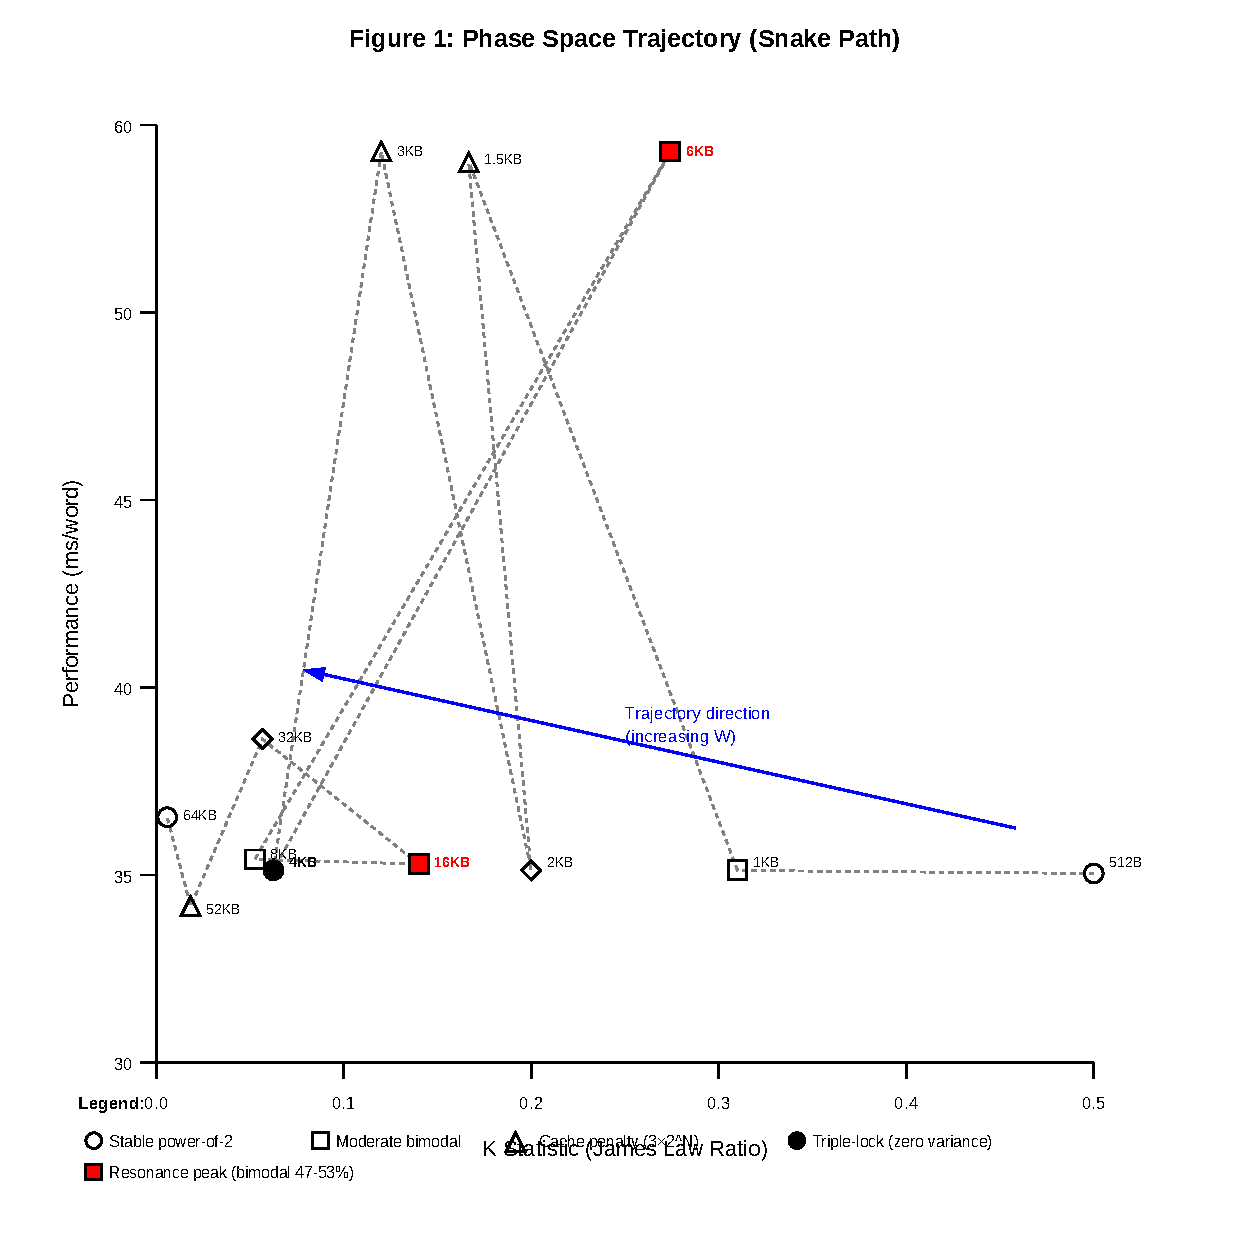
\includegraphics[width=0.8\linewidth]{../../working/papers/SSRN_companion/figures/fig1_snake_trajectory.pdf}
  \caption{Phase-space trajectory (snake plot).}
  \label{fig:snake}
\end{figure}
